\documentclass[12pt,a4paper,oneside,english]{book}

\usepackage{cite}

\usepackage[utf8]{inputenc}
\usepackage[T1]{fontenc}
\usepackage[english]{babel}
\usepackage{amsmath}
\usepackage{amsfonts}
\usepackage{amssymb}
\usepackage{graphicx}
\usepackage{subfig}
\usepackage{fancyhdr}
\usepackage{appendix}
\usepackage{hyphenat}
\usepackage{pdfpages}
\usepackage{float}
\usepackage{minitoc}
\usepackage[table]{colortbl}
\usepackage{lettrine}

\usepackage{array,multirow,makecell}
\newcolumntype{C}[1]{>{\arraybackslash}p{#1}}

\usepackage{enumitem}
\setlist{leftmargin=*,itemsep=0pt}

\usepackage{centernot}
\usepackage[linesnumbered,ruled,vlined,english,onelanguage]{algorithm2e}

\usepackage{quotchap}
\makeatletter
\renewcommand{\@makechapterhead}[1]{
 \chapterheadstartvskip
 {\size@chapter{\sectfont\raggedright
 {\chapnumfont
 \ifnum \c@secnumdepth >\m@ne
 \if@mainmatter\thechapter
 \fi\fi
 \par\nobreak}
 {\raggedright\advance\leftmargin10em\interlinepenalty\@M #1\par}}
 \nobreak\chapterheadendvskip}}
\makeatother
\renewcommand*{\chapterheadendvskip}{\vspace{2cm}}

\usepackage{geometry}
\geometry{hmargin=2.5cm,vmargin=2.5cm}

\pagestyle{fancyplain}
\lhead{\fancyplain{}{\nouppercase{\textit{\leftmark}}}}
\chead{\fancyplain{}{}}
\rhead{\fancyplain{}{}}
\lfoot{\fancyplain{}{}}
\cfoot{\fancyplain{}{}}
\rfoot{\fancyplain{\thepage}{\thepage}}
\renewcommand{\headrulewidth}{1pt}
\renewcommand{\footrulewidth}{1pt}
\setlength{\headheight}{15pt}

\renewcommand{\thesection}{\arabic{section}}

\usepackage{titlesec}
\titleformat{\paragraph}{\fontsize{11}{10}\bfseries}{\theparagraph}{1em}{}
\titlespacing*{\paragraph}{0pt}{10pt plus 2pt minus 0pt}{0pt plus 2pt minus 0pt}

\mtcsetfeature{minitoc}{before}{\vspace{-.5cm}}
\mtcsetfeature{minitoc}{after}{\vspace{-.5cm}}

\setcounter{secnumdepth}{4}
\setcounter{tocdepth}{4}

\usepackage{array}
\usepackage{multirow}
%\addto\captionsfrench{\def\tablename{\textsc{Tableau}}}

%\DefineBibliographyStrings{french}{urlseen = {},}

\setlength{\parskip}{8pt}
\usepackage{setspace}

\usepackage{url}



\usepackage{hyperref}
% Comment before printing to remove links' colors
\hypersetup{
 colorlinks,
 linktocpage=true,
 linkcolor=blue,
 citecolor=black,
 urlcolor=blue
 }

\sloppy

\author{GL4}
\title{Rapport PFA Facial Expression Recognition}

\begin{document}
\pagenumbering{gobble}

\includepdf[pages=-]{FrontPage.pdf}
\dominitoc
\mtcsettitle{minitoc}{Plan}
\mtcsetrules{*}{off}
\frontmatter
\spacing{1.4}
\chapter*{\textbf{Resumé}}
\normalsize{Ce projet a été créé dans le cadre d'un projet de fin d'année pour la deuxième année de Génie Logiciel à l'Institut National des Sciences Appliquées et de la Technologie. L'objectif de ce projet est de créer une extension de navigateur qui utilise un modèle de reconnaissance des expressions faciales construit à partir des techniques d'apprentissage profond et de vision par ordinateur.}

\medskip
{\noindent \textbf{Mots Clés: Apprentissage profond, Reconnaissance des expressions faciales, Vision par ordinateur, Extension de navigateur} }

{\let\clearpage\relax\chapter*{\textbf{Abstract}}}
\normalsize{This project was created as part of an end of the year project for the second year of Software Engineering at National Institute of Applied Sciences and Technology’s . The goal of this project is to create a browser extension that uses a facial expression recognition model built from deep learning and computer vision techniques.}

\medskip
{\noindent \textbf{Keywords: Deep learning, Facial emotion recognition, Computer vision, Browser extension} }

\spacing{1}

\tableofcontents
\newpage 
\listoffigures \mtcaddchapter 
\newpage 
\listoftables 
\newpage
\spacing{1.4}

\mainmatter
%\mtcaddchapter[Introduction générale] 
\chapter*{\textbf{General Introduction}}
\addcontentsline{toc}{chapter}{General Introduction}
\markboth{General Introduction}{}

\lettrine[findent=2pt]{\textbf{E}}{ }motional awareness is the ability to recognize and make sense of not just your own emotions, but also those of others. Facial expressions can display personal emotions and indicate an individual’s feeling within a social situation.
They are extremely important to the social interaction of individuals. If you only listen to what a person says and ignore what their face is telling you, then you really won't get the whole story. Often, words do not match emotions, and the face betrays what a person is actually feeling.

Therefore with the expansion of the machine learning field, and its contribution to almost all innovations. It is natural that we take full advantage of this technological evolution and exploit it into the Facial Expression Recognition field.

Some research have been made in this regard and some solutions have emerged during the years that consists of Macro-Facial Expression Detection using several algorithms and tools.

With the help of such solutions and information, we decided to build our model that will further enhance existing knowledge and deploy it into browsers via a chrome extension.

This report will be divided into four main chapters:
\begin{itemize}
\item[--] \textbf{Chapter 1: Project Context}

We will start this report with the general context of the project, the deep learning techniques related to the project and the different existing datasets.

\item[--] \textbf{Chapter 2: State of the Art}

In this section, we will identify existing solutions in this context, first by searching knows models and then the different deployed implementations to those models.

\item[--] \textbf{Chapter 3: Model Implementation}

In this chapter, we will explain the different phases that we went through to create our facial expression recognition model.

\item[--] \textbf{Chapter 4: Browser Extension Implementation}

In this last chapter, we will present how we deployed our model into an extension and then showcase the final results.

\item[--] Finally, we will close this report with a general conclusion on our project and opening a new perspective for further amelioration and upgrades.
\end{itemize}

\chapter{Project Context}
\label{ch:1er}
\minitoc
\newpage
\section*{Introduction}
This chapter is dedicated to present the context of the project. First, we show the different expressions that a face can have and the goal of our project then we move on to present existing deep learning models that serve this context. We close by making a comparison of different available datasets containing face images.

\section{Facial Expression Recognition}
We aim to provide a basic understanding of Facial Expression Recognition (FER) domain and define our goal for this project.
\subsection{Presentation}
\subsubsection{Definition}
Expressions reveal what takes place within the human mind at a time. These are either communicated by speech or displayed through facial movements and body gestures. Of all the known methods of expression, facial expressions are the foremost emotionally expressive.
A facial expression is a specific configuration of the micro-motors (small muscles) beneath the skin of the face.
For example, a smile to indicate happiness or agreement, a lowering of your brows to point out someone you're angry or frustrated.
\subsubsection{Classification}
Back in the late 1800s, Charles Darwin was the first person to notice that facial expressions are universal. He suggested that, like emotions, those expressions of emotions are innate and identical for every human being. At the time, his theory was discarded by the scientific community.
It wasn’t until the late 20th century that Dr. Paul Ekman and his team researched the subject and provided evidence to confirm Darwin's theory.
While each face has its own unique traits and way of presenting emotions, there are 7 universal expressions (+ neutral) shared by every human, regardless of age, race, gender, language, or religion.
\begin{figure}[H]
    \centering
    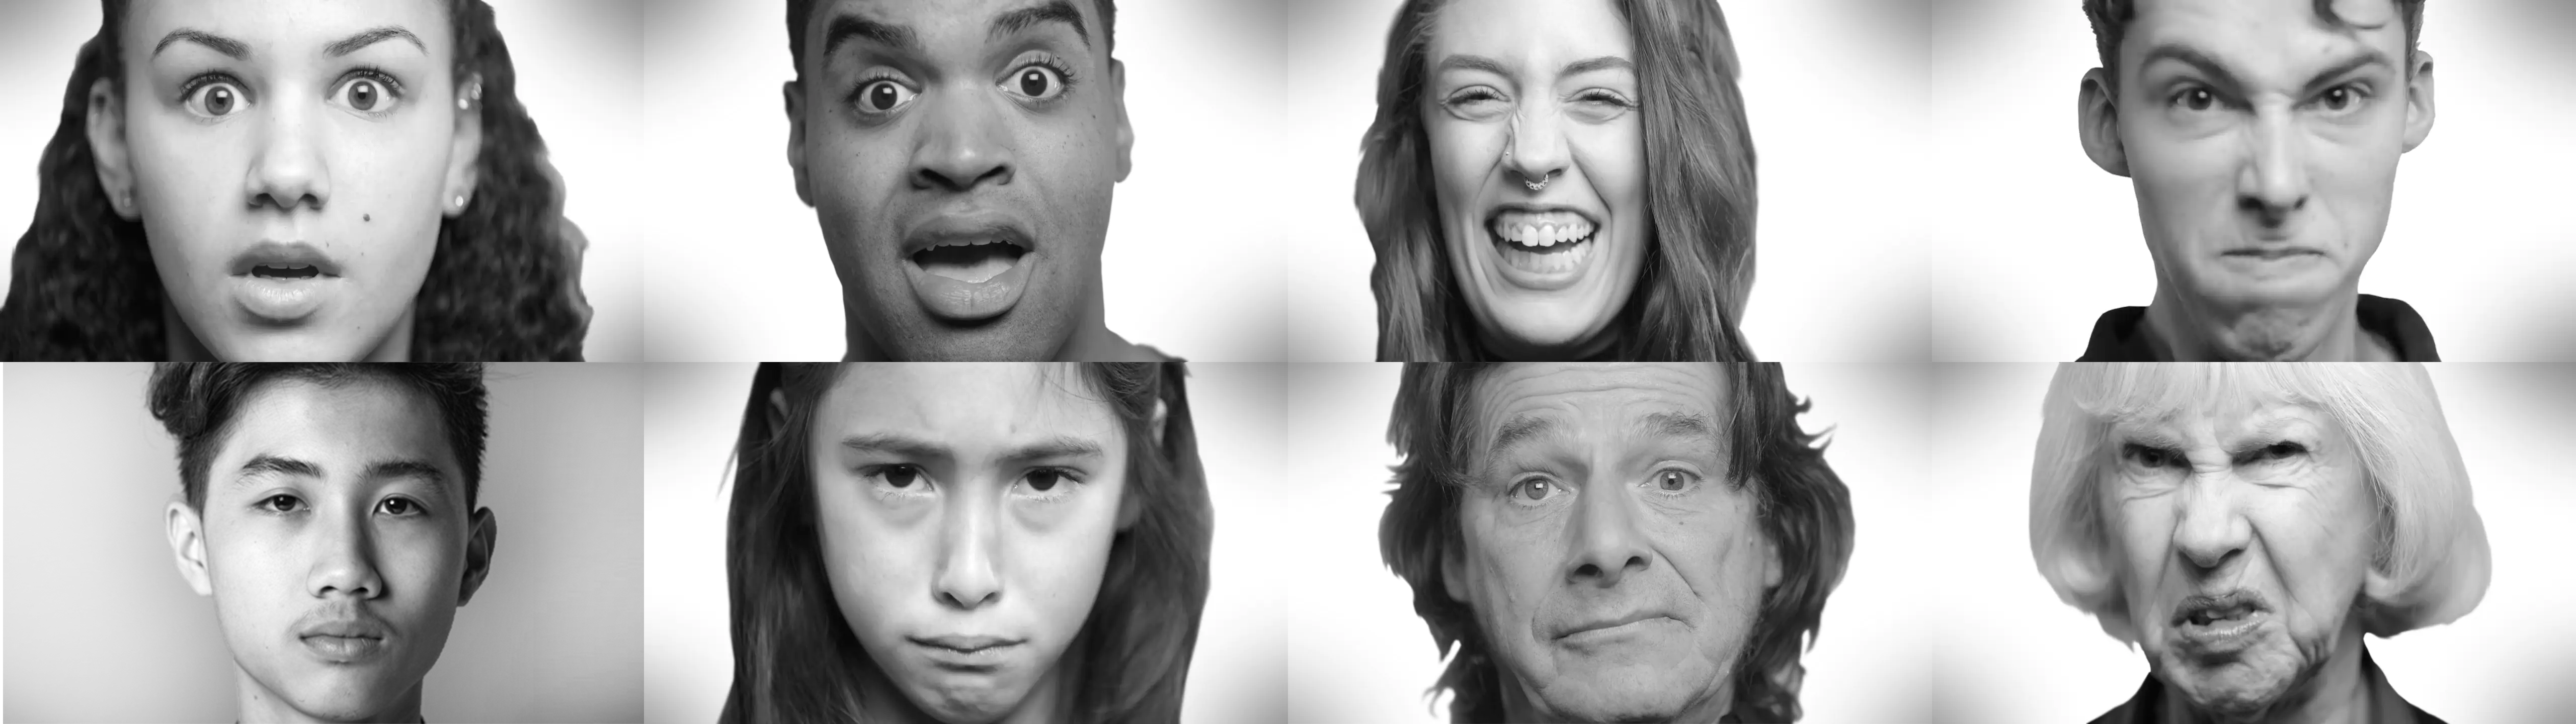
\includegraphics[width=0.9\textwidth]{figures/universal_expressions.png}
    \caption{Universal facial expressions}
    \label{fig:universalfer}
    \cite{universalFER}
\end{figure}
\noindent
From left to right of \autoref{fig:universalfer} we can list:

\begin{enumerate}
    \item Fear
    \\
    \hspace*{0.3cm}
    Eyebrows pulled up and together, upper eyelids pulled up, mouth stretched
    \item Surprise
    \\
    \hspace*{0.3cm}
    Entire eyebrow pulled up, eyelids pulled up, mouth hangs open, pupils dilated.
    \item Happiness
    \\
    \hspace*{0.3cm}
    The muscle around the eyes is tightened, “crows feet” wrinkles around the eyes, cheeks raised, lip corners raised diagonally.
    \item Anger
    \\
    \hspace*{0.3cm}
    Eyebrows pulled down, upper eyelids pulled up, lower eyelids pulled up, margins of lips rolled in, lips may be tightened.
    \item Neutral
    \\
    \hspace*{0.3cm}
    Micro-muscles relaxed.
    \item Sadness
    \\
    \hspace*{0.3cm}
    Inner corners of eyebrows raised, eyelids lose, lip corners pulled down.
    \item Contempt
    \\
    \hspace*{0.3cm}
    Eyes neutral with the lip corner pulled up and back on one side.
    \item Disgust
    \\
    \hspace*{0.3cm}
    Eyebrows pulled down, nose wrinkled, upper lip pulled up, lips loose.
\end{enumerate}

\subsection{Importance of Facial Expression Recognition}
Facial expressions are important factors in human communication that help us understand the emotions of others. They are not only manifestations of people's internal states; they are also clues for others to respond in a certain manner, providing universal hints for social coordination. Reading and understanding these emotions is the basis for empathy. Mastering this skill opens a window to our interlocutor's soul and mind.\\
Theses expressions are part of non verbal communication which makes 93\% of communication and it's absent when interacting with software and machines. Giving vision to the computer and making it recognize humans' expressions opens up a new realm of input that can be used in all sorts of ways in order to accommodate functionalities to their reactions. 

\section{Deep learning}
Deep Learning is a form of artificial intelligence, derived from Machine Learning. It is only recently, thanks to the advance in computing performance of computers, that this concept has developed. This learning attempts to model with a high level of data abstraction through articulated architectures of different nonlinear transformations. We’re interested in understanding convolutional neural networks and transfer learning methods.

\subsection{Convolutional Neural Network}

Convolutional Neural Networks (CNN) are distinguished from other neural networks by their superior performance with image, speech, or sound signal inputs. they need three main styles of layers, which are as follows:
\begin{enumerate}
    \item Convolutional layer
    \item Pooling layer
    \item Fully connected layer (FC)
\end{enumerate}

\begin{figure}[H]
    \centering
    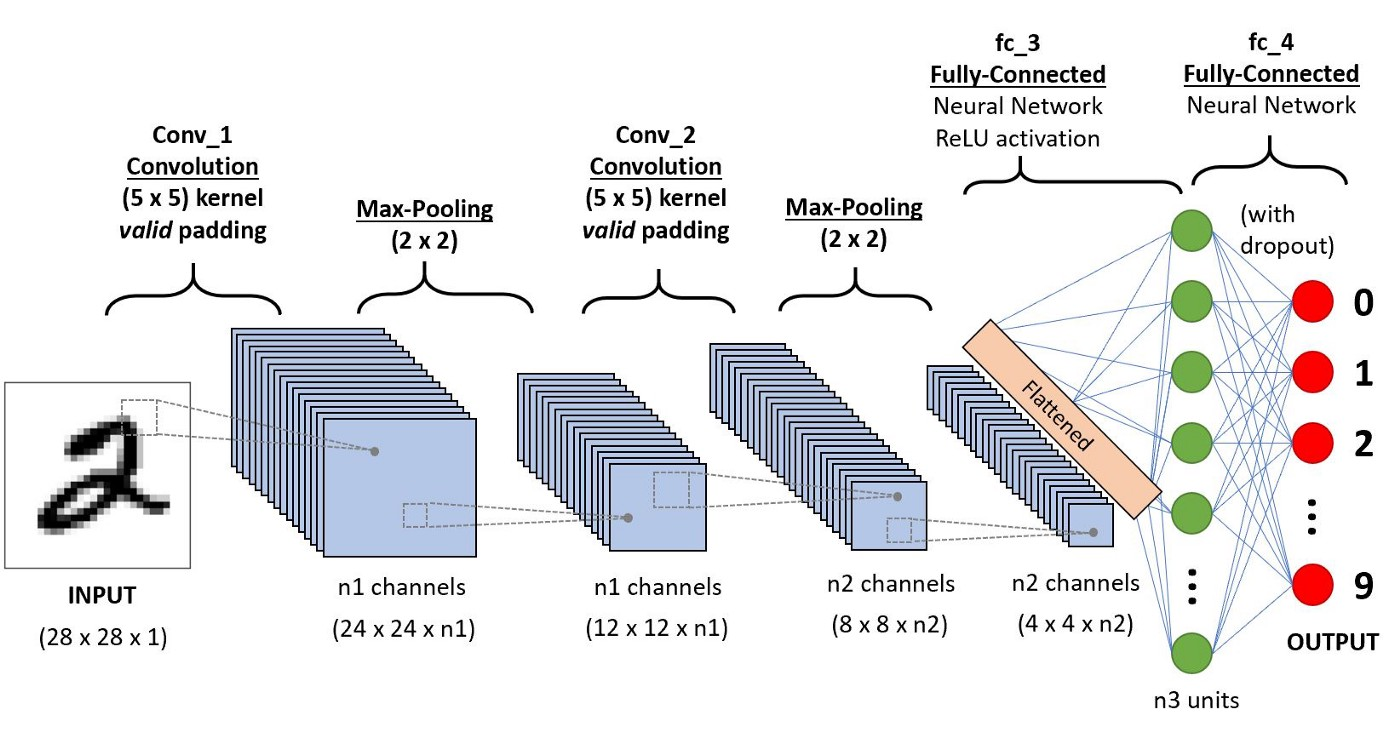
\includegraphics[width=0.7\textwidth]{figures/cnn_sequence.jpeg}
    \caption{A CNN sequence}
    \label{fig:cnn}
    \cite{cnnSequence}
\end{figure}

\subsubsection{Convolutional layer}
The convolution layer is the first layer in a CNN. It puts the input images through a collection of filters, each of which activates certain features from the pictures. A convolution converts all the pixels in its receptive field into one value. For instance, if you'd apply convolution to a picture, you'll be decreasing the image size further as bringing all the data within the field together into one pixel. As we go deeper within the network, we get more informative features and eliminate redundancy.

\begin{figure}[H]
    \centering
    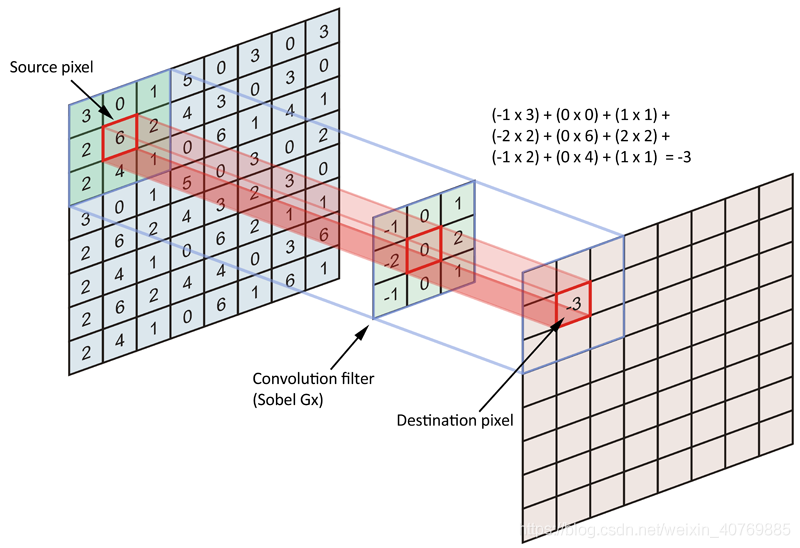
\includegraphics[width=0.7\textwidth]{figures/convolution_layer.png}
    \caption{Calculation of convolution}
    \label{fig:convolutional}
    \cite{convolutionLayer}
\end{figure}

\subsubsection{Pooling layer}
Pooling simplifies the output by performing nonlinear downsampling, reducing the quantity of parameters that the network has to learn. The first purpose of a pooling layer is to scale back the quantity of parameters of the input tensor and thus, help reduce overfitting, extract representative features from the input tensor and reduce computation and thus aid efficiency. The foremost popular style of pooling operation is max pooling, which extracts patches from the input feature maps, outputs the most value in each patch, and discards all the other values.

\begin{figure}[H]
    \centering
    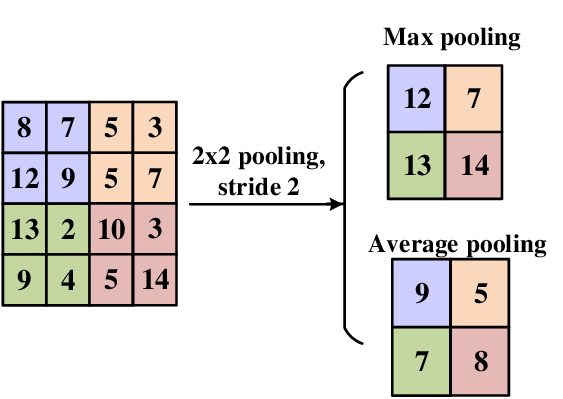
\includegraphics[width=0.5\textwidth]{figures/PoolingLayer.png}
    \caption{Pooling layer operation}
    \label{fig:pooling}
    \cite{poolingLayer}
\end{figure}

\subsubsection{Fully connected layer}
A Fully Connected Layer is solely feed-forward neural networks. FC Layers form the last few layers within the network. The input to the fully connected layer is the output from the ultimate Pooling or Convolutional Layer, which is flattened and so fed into the fully connected layer. This Flattened vector is then connected to some fully connected layers. For every layer of the artificial neural network, the subsequent calculation A(Wx + b) takes place,  where :
\begin{itemize}
    \item x : the input vector 
    \item W : the weight 
    \item b : the bias vector which is responsible for shifting the function in an order that isn't constrained to the origin.
    \item A : Activation function

\end{itemize}
This calculation is repeated for every layer. After passing through the fully connected layers, the final layer uses an activation function which is used to get probabilities of the input being in a particular class (classification problem). Finally, we get the probabilities of the object belonging to the different classes we have.

\begin{figure}[H]
    \centering
    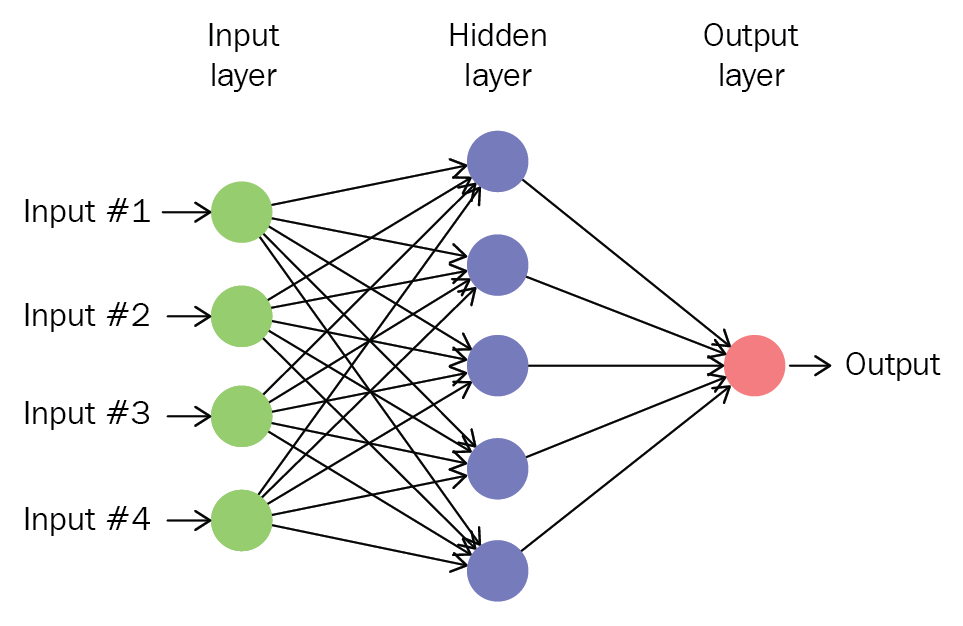
\includegraphics[width=0.6\textwidth]{figures/fullyConnectedLayers.png}
    \caption{Fully connected layer}
    \label{fig:fullyConnected}
    \cite{fullyConnected}
\end{figure}

\subsection{Transfer Learning}
Transfer learning is a machine learning approach in which a model that was developed for a task is reused as the starting point for a model on a second task.
It's a well-known method in deep learning where pre-trained models are used as the starting point for computer vision and natural language processing tasks. Given the large computing and time resources required to develop neural network models, the pre-trained models provide a head start on correlated problems.
In what follows we will mention some of the most famous models employed with transfer learning for CNNs.

\subsubsection{VGG-19}
VGG is a deep CNN used to classify images. VGG is the successor of AlexNet but it was created by a different group named Visual Geometry Group at Oxford, It carries some ideas from its predecessors, but also adds deep Convolutional neural layers to improve accuracy. VGG-19 is a variant of the VGG model which in short consists of 19 layers (16 convolution layers, 3 fully connected layers, 5 MaxPool layers, and 1 SoftMax layer). There are other variants of VGG like VGG11 and VGG16.
\begin{figure}[H]
    \centering
    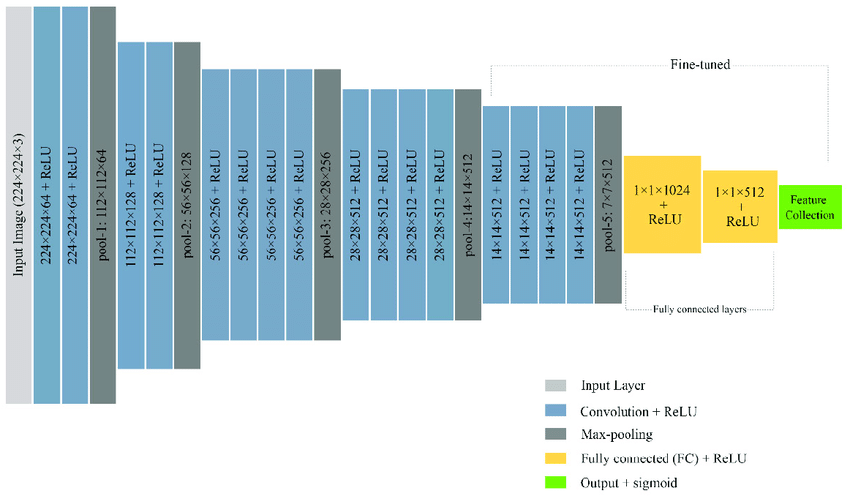
\includegraphics[width=0.7\textwidth]{figures/Illustration-of-fine-tuned-VGG19-pre-trained-CNN-model.png}
    \caption{Illustration of a fine-tuned VGG-19 model.}
    \label{fig:vgg}
    \cite{vgg19}
\end{figure}
\noindent

\subsubsection{Resnet}
When it comes to convolutional neural networks, researchers affirm that “the deeper the better”, However, it has been noticed that after some depth, the performance degrades. Here come ResNets to solve this famous problem known as vanishing gradient, introducing the skip connection as a solution concept.
The basic idea of this solution named skip connection is to direct the input of a layer and add it to the output after some layers. This provides more information to the layer and helps in a way to overcome the vanishing gradient problem.

\begin{figure}[H]
    \centering
    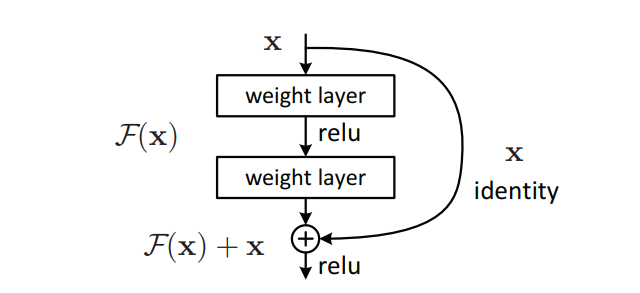
\includegraphics[width=0.7\textwidth]{figures/Residual-Block.png}
    \caption{Skip (shortcut) connection}
    \label{fig:resnet}
    \cite{resnet}
\end{figure}
\noindent


\section{Datasets}
In this third section of our project context, we describe various data sources containing facial expressions and compare them to make the best choice for our project.

\subsection{Sources}
During our search for an appropriate dataset of facial expressions for our project, we found many publicly available sources. Below, we list and compare four most commonly used databases, primarily based on their size, their diversity and their properties.

\subsubsection{FER2013: Facial Expression Recognition 2013 Dataset } 
This Kaggle dataset was released in 2013 during the competition of “Facial Expression Recognition Challenge” \cite{ferData}. It was prepared by Pierre-Luc Carrier and Aaron Courville, as part of an ongoing research project. It contains over 30K grayscale facial images labeled with 7 expressions. It’s fairly balanced between all the emotions, except for “disgust” which covers only 1.82\% of the dataset.

\subsubsection{CK+ : Extended Cohn Kanade dataset }
The Cohn-Kanade (CK) dataset\cite{ckData} was published in 2000 and since then it has become widely used for algorithm development. It has 593 video sequences recorded at 30 frames per second, saved as a series of successive frames for each video which brings it to a total of 5876 images, all of them labeled with one of 7 expressions labels.

\subsubsection{Affect Net}
Affect Net\cite{affectNetData} was created by professors at the university of Denver in order to overcome the limitations of other small datasets. It has more than 1 million facial images. They were collected from the internet using keywords related to emotions in 6 languages. The majority of these images were manually labeled with the appropriate emotion and its intensity and the intensity of arousal. It’s a unique work with an increasing popularity each year.

\subsubsection{Google facial expression comparison dataset }
This dataset was composed by Google Research \cite{googleData} with face images taken from Flickr. The images are grouped in triplets and it specifies which pair are the most similar of each triplets. 6 raters helped annotate this dataset which contains around 500K triplets formed from 156K face images.

\subsection{Comparison}
To make things clearer, we collected and organized all the important informations about these datasets in \autoref{tab:datasets}. We will be using it in the third chapter.\newline

\begin{table}[H]
\begin{tabular}{|c|c|c|c|c|}
\hline
\textbf{Data source} & \textbf{FER2013} & \textbf{CK+} & \textbf{Affect Net} & \textbf{Google FEC} \\
\hline
\textbf{Year} & 2013 & 2000 & 2017 & 2018 \\ 
\hline
\textbf{Number of images} & 32,298 & 593 & 1 000 000 & 156 000\\ 
\hline
\textbf{Image size} & 48*48 & 640*480 & variable & variable \\ 
\hline
\textbf{Format} & .jpg images & 30 fps videos & - & .csv of image URLs \\
\hline
\textbf{File size} & 56 MB & 158 MB & 120 GB & 200 MB \\ 
\hline
\multicolumn{1}{|p{2.5cm}|}{\nohyphens{\textbf{Facial expressions labels}}} & \multicolumn{1}{p{2.5cm}|} {7: Anger, Disgust, Fear, Happiness, Sadness, Surprise, Neutral }& \multicolumn{1}{p{2.5cm}|} {7: Anger, Disgust, Fear, Happiness, Sadness, Surprise, Contempt} & \multicolumn{1}{p{2.5cm}|}{ 8 emotions +intensity of valance +intensity of arousal} & \multicolumn{1}{p{2.5cm}|}{30 emotions} \\ 
\hline
\textbf{Easily accessible?} & Yes & Yes & No & Yes \\ 
\hline
\end{tabular}
\caption{Comparison of facial images datasets’ properties}
\label{tab:datasets}
\end{table}

\section*{Conclusion}
This chapter gave us the occasion to put our project in its frame, we presented the 7 main universal expressions at first. We also explained CNN and Transfer Learning methods in deep learning. Finally, we concluded this chapter with a comparison of available face datasets.
In the next chapter, we will be presenting the existing solutions.

\addtocontents{toc}{\protect\newpage}
\chapter{State of art}
\label{ch:2eme}
\minitoc
\newpage
\section*{Introduction}
In this chapter, we are going to search existing solutions that use facial expression recognition.
In the first part, we are going to research known models. In the second part, we will be exploring deployed implementations. Then we will state our goals.
\section{FER Models}
\subsection{Convolution Neural Network}
\subsubsection{Coursera}
We found a guided project in Coursera, taught by Snehan Kekre, a machine learning instructor \cite{courseraProject}.
In his course, he proposed a sequential CNN architecture.
\begin{figure}[H]
    \centering
    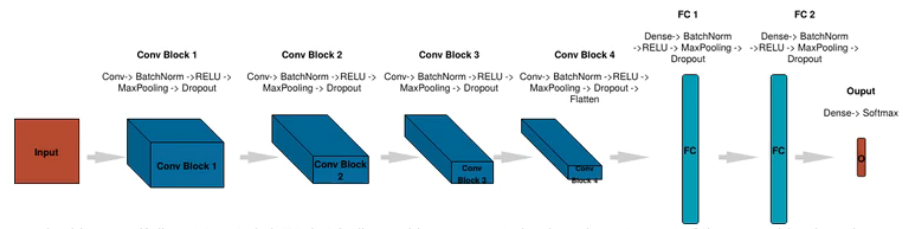
\includegraphics[width=1\textwidth]{figures/State of art/coursera_CNN_architecture.png}
    \caption{Coursera CNN architecture}
    \label{fig:coursera1}
\end{figure}
\noindent
He designed 6 activation layers, 4 convolution layers and 2 fully controlled layers.
The ReLu function is used to increase the non-linearity in the images. Max-pooling is used for dimensions reduction of the image. Dropout function is to avoid overfitting the training data. Flatten to convert image to a 1-dimensional array. 1-dimensional array becomes the input to the fully controlled layers. Output layer has two techniques, dense and soft-max.
\newline
To study the accuracy of the model, the metrics are set to accuracy.
The loss is set to categorical cross-entropy as the data has to be classified into only the 7 defined categories and each image can belong to one classification type only.
\newline
After training the model for 15 epochs, on the FER-2013 dataset, he gets an accuracy of 66.7\%

\subsubsection{DeepFace}
DeepFace \cite{deepface} is a lightweight deep face recognition and facial attribute analysis (age, gender, emotion and ethnicity) library for Python, written by Sefik Ilkin Serengil.The project passed 3K\texttt{+} stars on GitHub and 350K\texttt{+} installs on pip / pypi.\\
Training the model on the FER-2013 dataset, he obtained a 57.42\% accuracy
\begin{figure}[H]
    \centering
    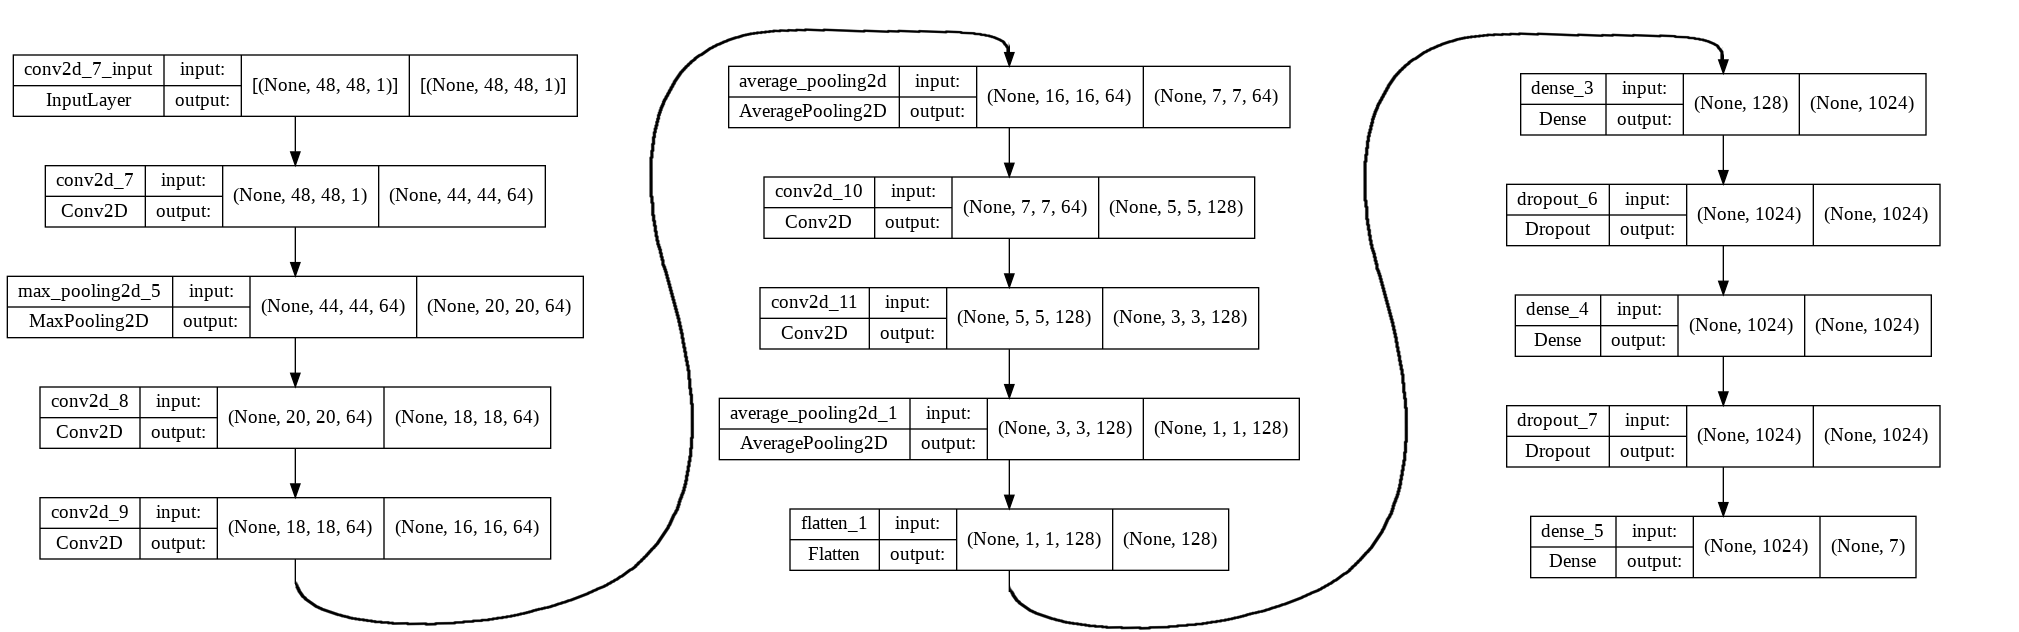
\includegraphics[width=1\textwidth]{figures/State of art/DeepFacemodel.png}
    \caption{DeepFace CNN model architecture}
    \label{fig:deepface}
     \cite{deepfacearticle}.
\end{figure}
\noindent


\subsection{Transfer learning}
\subsubsection{VGG-19}
The proposed system consists of the following steps: pre-processing, feature extraction, feature selection, and classification. Using the CK\texttt{+} dataset, the grayscale images are pre-processed by resizing the shape and performing intensity normalization on the pixel values. These images are given as input to the pre-trained VGG19 network. After extracting the features, Principal Component Analysis (PCA) is performed on each set in order to reduce the dimensions. Finally, a linear Support Vector Machine (SVM) classifier is used to output the class label of the predicted facial expression.\\
Since the dataset is small, a 10 fold cross validation is performed, achieving an accuracy of 92.26\%.
\begin{figure}[H]
    \centering
    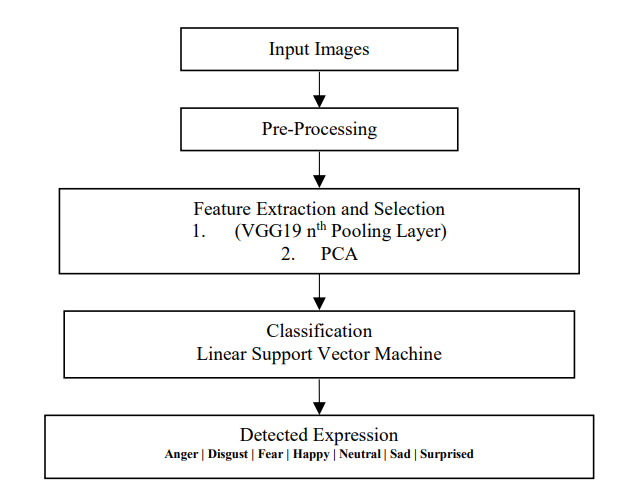
\includegraphics[width=0.5\textwidth]{figures/State of art/vggmodelarchitecture.PNG}
    \caption{VGG-19 FER training model implementation.}
    \label{fig:vgg19architecture}
    \cite{vgg19article}
\end{figure}
\noindent


\subsubsection{Resnet-50}
ResNet-50 is a pre-trained model for image classification using CNN. Composed of convolution and pooling layers, responsible for local amplification and local feature extraction. A FC layer is then added, for feature weighting and flattening. A soft-max is used in the end for classification. The dataset adopted is specifically created for this experiment and contains 700 images collected by a professional photographer. A 10 fold cross validation is performed, achieving an average accuracy of 95.39±1.41\%. 
\begin{figure}[H]
    \centering
    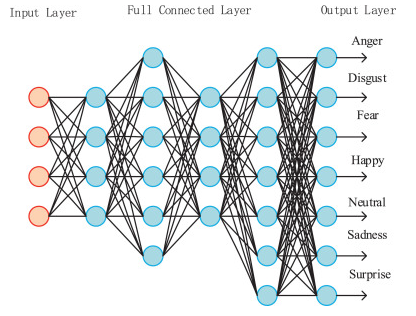
\includegraphics[width=0.6\textwidth]{figures/State of art/resnet50model.png}
    \caption{Resnet-50 model implemented in FER.}
    \label{fig:resnet50article}
    \cite{resnet50article}
\end{figure}
\noindent


\section{Implementations}
\subsection{Chrome extension - Blissify}
Blissify is an extension for Google Chrome that uses emotion detection technology. Using the user's webcam, it will monitor the facial expressions in real-time as he browses the internet and block the websites upon detecting a rapid increase in negative emotions.
\begin{figure}[H]
    \centering
    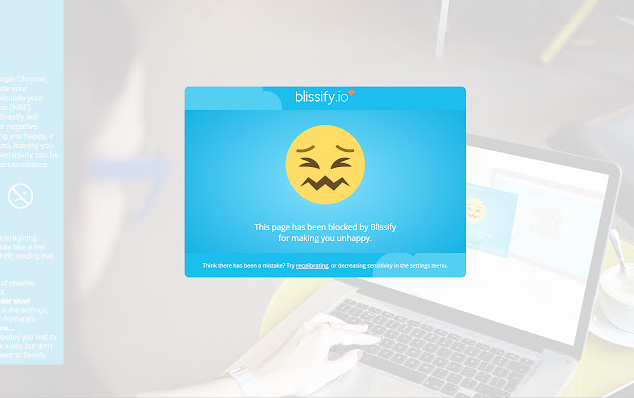
\includegraphics[width=0.6\textwidth]{figures/State of art/blissify.PNG}
    \caption{Blocked website by blissify}
    \label{fig:blissify}
    \cite{blissify}
\end{figure}
\subsection{Surveillance system - Xeoma}
Xeoma’s surveillance system implements FER to monitor people and recognize negative emotions.
By recognizing the mood of the crowd, vandalism and conflicts can be prevented at events and in public places such as an airport or a concert.
Moreover, by recognizing customers’ emotions, companies can improve the quality of service and client-oriented approach by analyzing the results of an advertising campaign showing the emotions of visitors that come to the banner ad for example.
\begin{figure}[H]
    \centering
    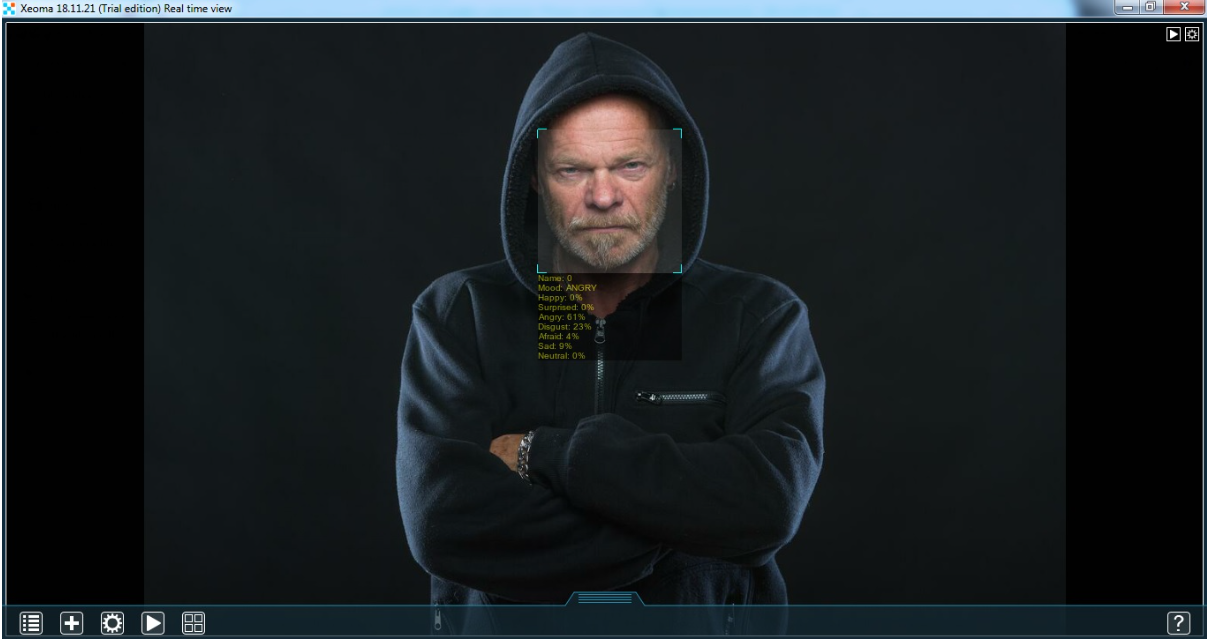
\includegraphics[width=0.6\textwidth]{figures/State of art/xeoma.PNG}
    \caption{Face emotion detector by Xeoma surveillance system}
    \label{fig:xeoma}
    \cite{xeoma}
\end{figure}
\subsection{Child education mobile application - 4littletrees}
4littletrees's mission is to solve the real-world challenges in traditional education by developing novel artificial intelligence (AI) technologies to provide an adaptive and personalized learning experience for students worldwide. This is achieved by detecting and identifying the learners’ emotions and performance in real-time to understand where they struggle on a particular subject.
\begin{figure}[H]
    \centering
    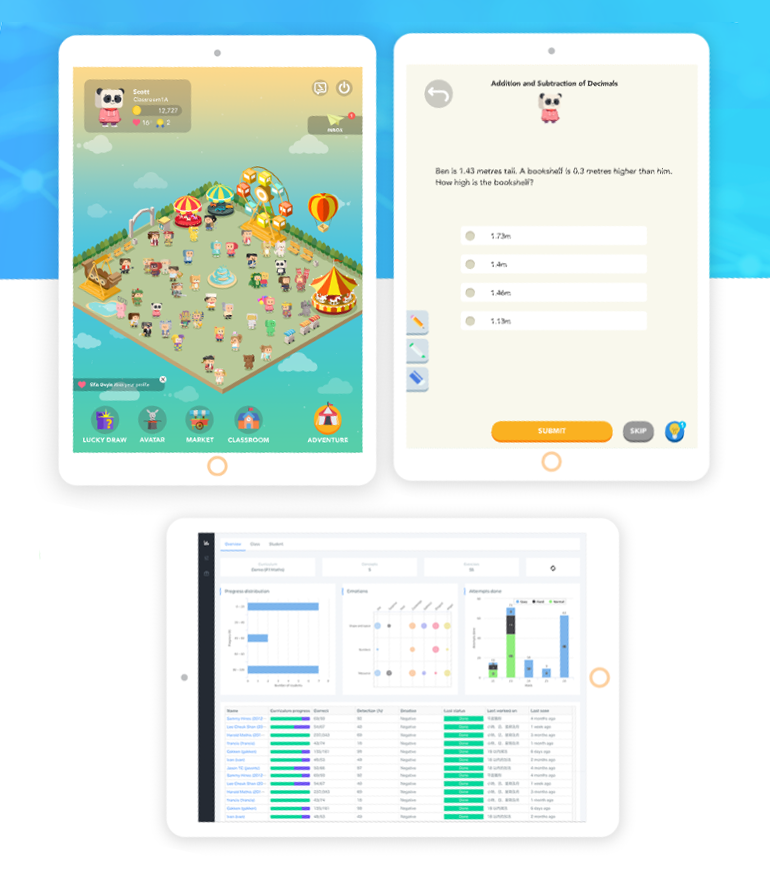
\includegraphics[width=0.55\textwidth]{figures/State of art/4littletrees.PNG}
    \caption{4littletrees exercises and data analysis board}
    \label{fig:4littletrees}
    \cite{4littletrees}
\end{figure}
\noindent
Two main functionalities are offered: 
\begin{itemize}
    \item Alerting students and getting their attention back when they are off track.
    \item Measuring their facial expressions and emotions and generating detailed reports for teachers.
\end{itemize}

\subsection{Video editor - Morphcast}
Morphcast is a video editor, that integrates Facial Emotion AI technology in order to create interactive videos triggered by viewers' emotions. It allows users to boost engagement by customizing the content, based on the emotions, attention level, engagement, and many other unique traits of each individual viewer.
\begin{figure}[H]
\begin{center}
\subfloat[]{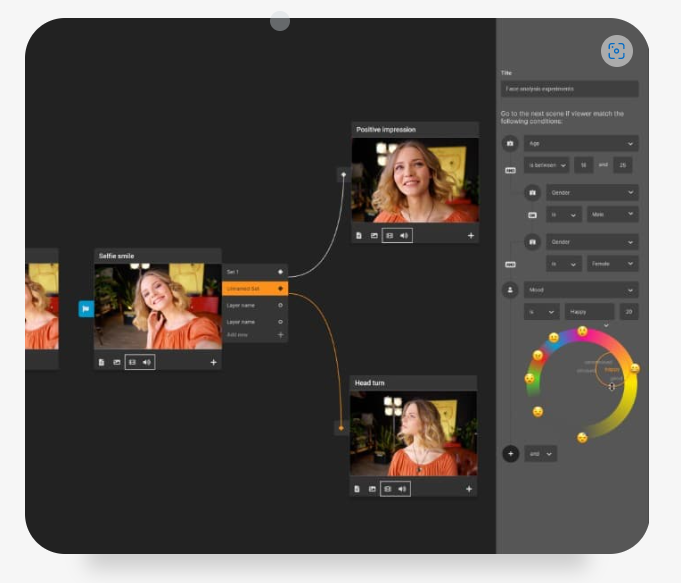
\includegraphics[width=0.4\textwidth]{figures/State of art/morphcast.PNG}\label{fig:morphcast1}}\quad 
\subfloat[]{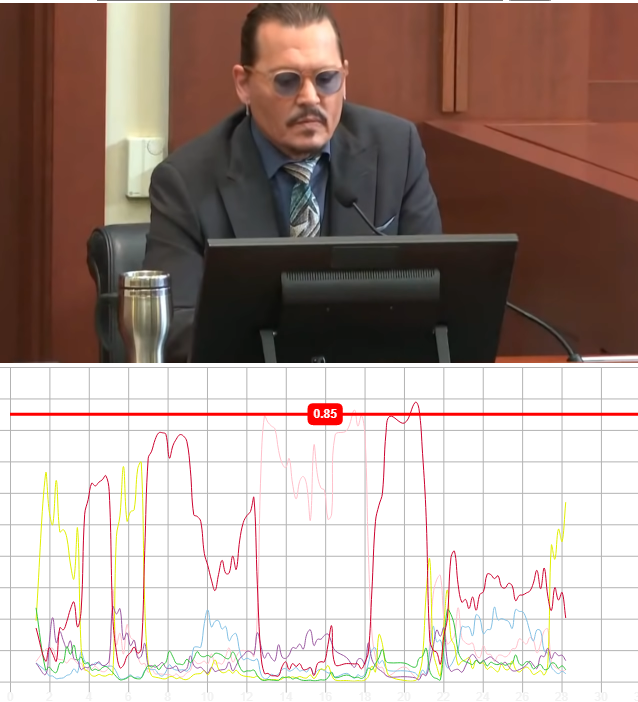
\includegraphics[width=0.4\textwidth]{figures/State of art/morphcast_test.png}\label{fig:morphcast2}}
\caption{Mophcast editing phase and emotional tracking}
\label{fig:morphcast}
\cite{morphcast}
\end{center}
\end{figure}


\noindent
  The platform allows businesses and creators to collect emotional data while the viewer is watching the video, whether it is an advertising video, a tutorial, a presentation, or any other kind of content. This feature gives a throughout insight on their reactions and thoughts, which dramatically increase customers’ engagement and establish a stronger relationship with the audience.

\section{Our goals}
After this research of the state of art, we wanted to implement a new nonexistent solution with the best performing model.\\ \\
Our first goal is to benchmark the models to study their performances and accuracy then optimizing the best one. This is an important step because we want to make sure that expressions are detected accurately most of the time. Reaching a perfect model is near impossible but we strive to use the existing knowledge and enhance it. We will then use this model to predict facial expressions.\\ \\
Our second goal is to develop a browser extension with this model. In fact, browser extensions are accessible and easy to use by anyone. They are also feasible to produce. We want to offer the possibility for everyone to analyze the emotions of an interlocutor. It can either be from a video call or a speaker in a Youtube video. We believe that giving this freedom of choice to the user is very important to cover everyone's needs.
\section*{Conclusion}
This chapter gave us a clear vision on the field of FER. We presented 4 models used for FER, two of them are based on CNN and the other two on transfer learning. We found 4 implementations, each one with a different use case and platform. They helped us visualize a new solution which consists of a chrome extension that utilises a FER model to give a summary of emotions while navigating the web. In the next chapter, we will be presenting our model implementation.

\chapter{Model Implementation}
\label{ch:3eme}
\minitoc
\section*{Introduction}
After researching the available datasets and models, we can now move on to work on a model for FER that will be used in our web browser extension. We will first present the software environment, as well as the technologies . Also, we will present the chosen dataset and the preprocessings we performed on it. Then, we will train different models on this dataset. Finally, we will show the test results of the chosen model.
\section{Used tools}
In this section, we describe our development environment of choice and what technologies we will be using in order to train the models.
\subsection{Training environment}
First, we started training models locally on our laptops, using its hardware (CPU, GPU and RAM). We configured their environment and installed the needed modules but we encountered multiple problems that hindered our progress: Model training is slow and it crashes randomly due to the weak available hardware we got. \\
We then decided to move our work to a cloud based solution and we used Google Colab.
\\
\\
\textbf{Google Colab}\cite{googlecolab} is a free research tool for research related to automatic learning, based on a Jupyter notebook environment which doesn't require prior configuration. The code is executed on a dedicated virtual machine to the user. Although it is freely accessible, it presents limits such as limited RAM and runtime, but it offered the needed stability for our model training.
\newpage


\subsection{Language and libraries}
We will present the main technologies we used to train the models.
\begin{itemize}
\item Python \cite{python}: is an interpreted, high-level, dynamic programming language, widely adopted by the data science community. In fact, it has libraries dedicated to the different stages data science projects, such as Pandas, Matplotlib, scikitlearn, as well as advanced libraries such as TensorFlow and Keras for deep learning.
\item Keras \cite{keras}: is a high-level neural network API, written in Python and associated with TensorFlow. It was developed with the objective of allowing rapid experimentation on deep neural networks.
\item Matplotlib \cite{matplotlib}: is a 2D plotting library in Python that produces figures of quality for publications on all platforms, in a variety of formats and interactive environments.
\item Livelossplot \cite{livelossplot}: is a 2D plot callback in Jupyter Notebook that is used by Keras and PyTorch. It plots a live training accuracy while training the model by many epochs.
\end{itemize}

\section{Used dataset}
In this section, we will go over the datasets used for the FER that we introduced back in chapter 1, and decide which one we're going to base our model training on then we're going to preprocess.

\subsection{Selection}
Looking at the comparison table at \autoref{tab:datasets}, we notice that each dataset is unique in all the stated criteria. We based our choice on elimination depending on our needs.
\begin{itemize}
\item Affect Net is the one with the biggest number of images. A bigger dataset means a slower training but more accurate results. The drawback that it's very huge (120 GB) and it isn't accessible to the public.
\item Google FEC is a recent fairly big dataset with 156 000 images. The problem is that images are grouped in triplets and are labeled with 30 expressions which doesn't suit our need of macro facial expressions for the browser extension.
\item CK\texttt{+} is an old dataset with high quality images which explains its popular use. But the number of images is too small and they are repeated since they are frames of videos, which causes eventual overfitting.
\item FER2013 contains small grayscale images taken from the wild but it is enough to train a GER, plus it's a big freely available dataset.
\end{itemize}
In the end, we chose \textbf{FER2013} to test different models and to improve the results, we're going to preprocess it by cleaning it and augmenting it.

\subsection{Preprocessing}
We will first present the FER2013 dataset then suggest how we're going to improve it.
\subsubsection{Overview}
FER2013 is a dataset of 35887 grayscale face images with the same dimension of 48 x 48 pixels that was shared for the Kaggle competition in 2013. Anger, happiness, sadness, surprise, fear, neutral, and disgust are the 7 basic types of facial expressions found in this dataset. \autoref{fig:fer_overview} shows a sample of these images.
\begin{figure}[H]
    \centering
    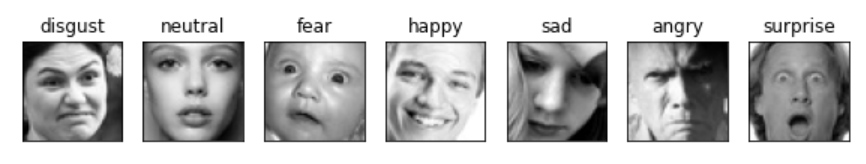
\includegraphics[width=0.9\textwidth]{figures/model/feroverview.jpg}
    \caption{Fer2013 image sample for each emotion}
    \label{fig:fer_overview}
\end{figure}
\noindent
The images are separated into 2 folders, 28709 in train and 7178 in test. Each one of them contains 7 folders for each expression. \autoref{fig:fer13traintest} depicts the distribution of images. We can see that the images labeled happy take the biggest portion of the dataset while images labeled disgust take the smallest.
\begin{figure}[H]
\begin{center}
\subfloat[]{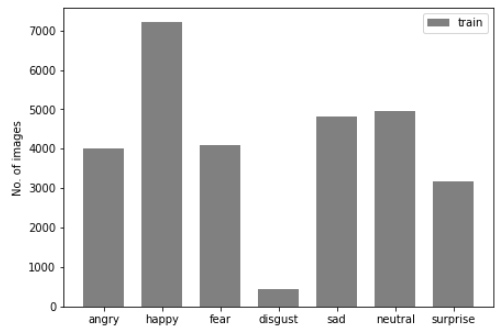
\includegraphics[width=0.4\textwidth]{figures/model/fer13train.jpg}}\quad 
\subfloat[]{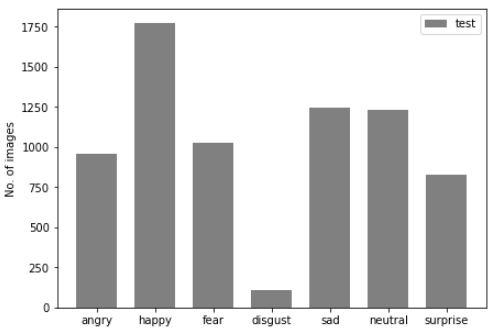
\includegraphics[width=0.4\textwidth]{figures/model/fer13test.jpg}}
\caption{FER2013 Distribution}
\label{fig:fer13traintest}
\end{center}
\end{figure}

\subsubsection{Data cleaning}
Even though this dataset is big, not every image is a valid image. When we checked the folders, we found cartoon characters, images with thick watermark over the face, blank images and images with the wrong facial expression (like a happy face in sad folder). After realising this, we went to clean the data and delete these images manually. \autoref{fig:fer_wrongdata}
\begin{figure}[H]
    \centering
    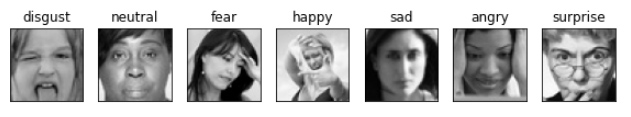
\includegraphics[width=0.9\textwidth]{figures/model/ferwrongdata.jpg}
    \caption{a Sample of Fer2013's inaccurate images}
    \label{fig:fer_wrongdata}
\end{figure}
\noindent
In addition, since we don't have enough images for the disgust expression, we decided to remove it so it doesn't disrupt the training of the other 6 emotions.
We have now a total of 31,247 images, with 24217 in train and 7030 in test. Then we uploaded this cleaned dataset to Kaggle so we could use it later in google colab.
\autoref{fig:fercleantraintest} shows the newly distribution of images for training and for testing.
\begin{figure}[H]
\begin{center}
\subfloat[]{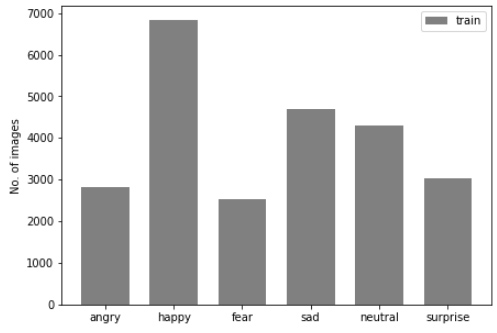
\includegraphics[width=0.4\textwidth]{figures/model/fercleantrain.jpg}}\quad 
\subfloat[]{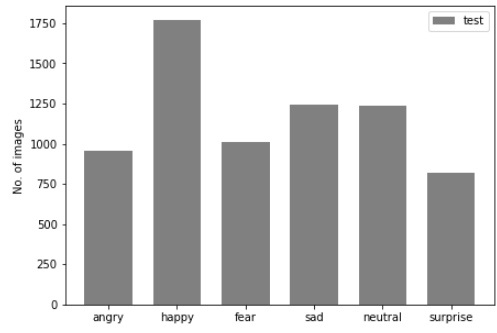
\includegraphics[width=0.4\textwidth]{figures/model/fercleantest.jpg}}
\caption{Clean FER2013 Distribution}
\label{fig:fercleantraintest}
\end{center}
\end{figure}

\subsubsection{Data augmentation}
Data augmentation is a technique that increases the size of a dataset without having to
collect new data by providing some variation to the photos. Since FER2013 images are small, it is beneficial to use this technique to enhance them. We have augmented our data with a horizontal flip and 10 ranges of zoom, rotation, shear and shift transformations. The \autoref{fig:data_augmentation} shows the portion of
code that we have used for the data augmentation to preprocess our datasets.
\begin{figure}[H]
    \centering
    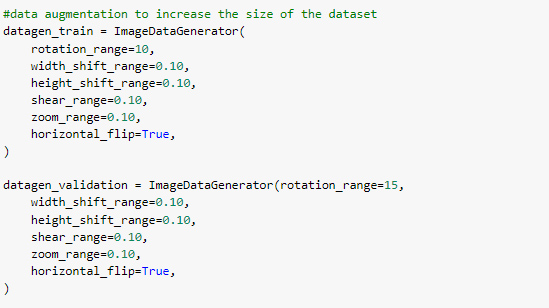
\includegraphics[width=0.8\textwidth]{figures/model/data augmentation.jpg}
    \caption{Data augmentation code with ImageDataGenerator}
    \label{fig:data_augmentation}
\end{figure}

\section{Training and testing}
After preparing our data, we used it to train 4 different models. Here are general common parameters we used to configure the training:
\begin{itemize}
\item A batch size of 32.
\item Categorical cross entropy as the loss function because we are classifying multiple classes.
\item Adam optimizer to optimize the loss function with a learning rate of 0.0001
\item We tracked the accuracy and loss through each epoch, for training and validation. A live graph is shown with livelossplot.
\end{itemize}
For each model, we will be showing 2 graphs, one for accuracy and one for loss, having 2 plots. Blue plot is for training, orange plot is for validation.

\subsection{Cousera}
\begin{figure}[H]
    \centering
    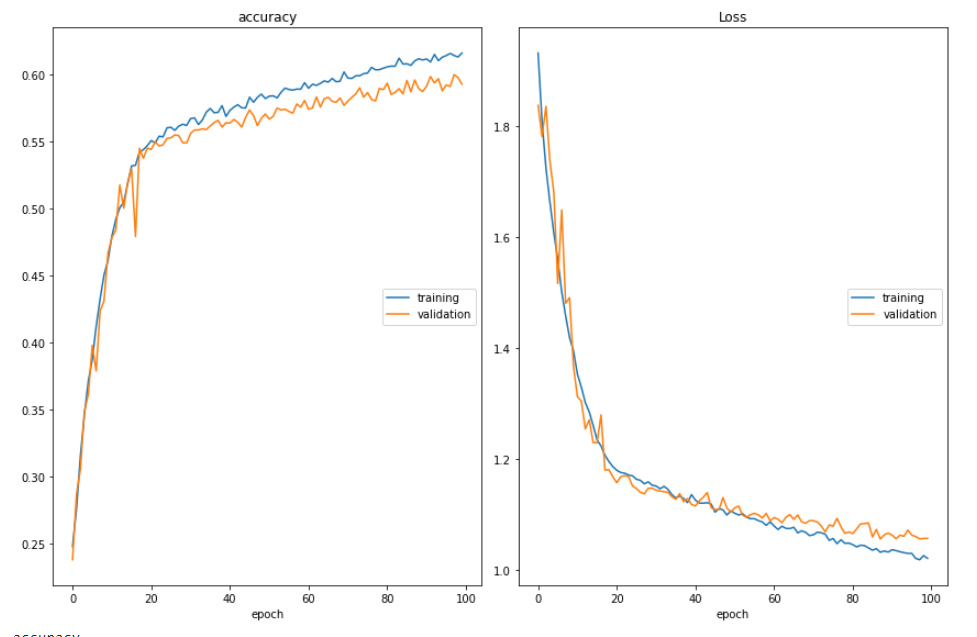
\includegraphics[width=0.6\textwidth]{figures/model/courseragraph.jpg}
    \caption{Training results of the Coursera model}
    \label{fig:courseragraph}
\end{figure}
\noindent
We ran this model for 20 epochs and it showed great results. Training and validation accuracy were increasing together. We redid the training with 100 epochs and the behaviour didn't change. We reached a training accuracy of 61.6\% and a validation accuracy of 59.2\%. Both are close and didn't converge yet. Even the loss is decreasing. The model is extracting features from the dataset and isn't overfitting and it could do better with more epochs.
\subsection{DeepFace}
\begin{figure}[H]
    \centering
    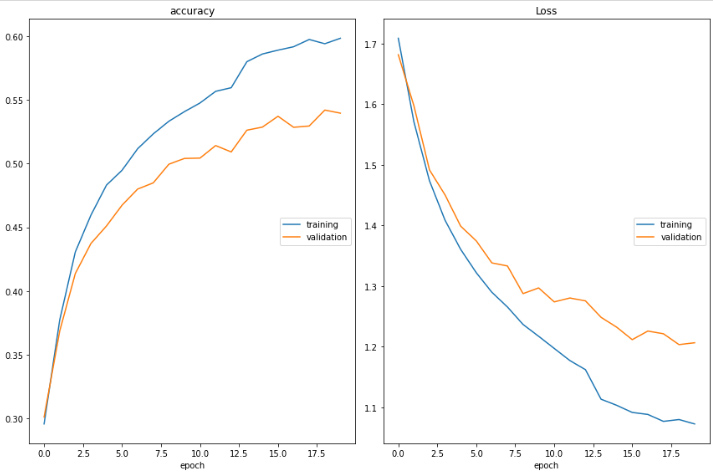
\includegraphics[width=0.6\textwidth]{figures/model/deepfacegraph.jpg}
    \caption{Training results of the DeepFace model}
    \label{fig:deepfacegraph}
\end{figure}
\noindent
We ran this model for 20 epochs. We reached a training accuracy of 59.9\% and a validation accuracy of 54.2\%. Starting from epoch 5, they began to diverge from each other. There is no sign of fluctuations but DeepFace is overfitting the data.

\subsection{VGG-19}
\begin{figure}[H]
    \centering
    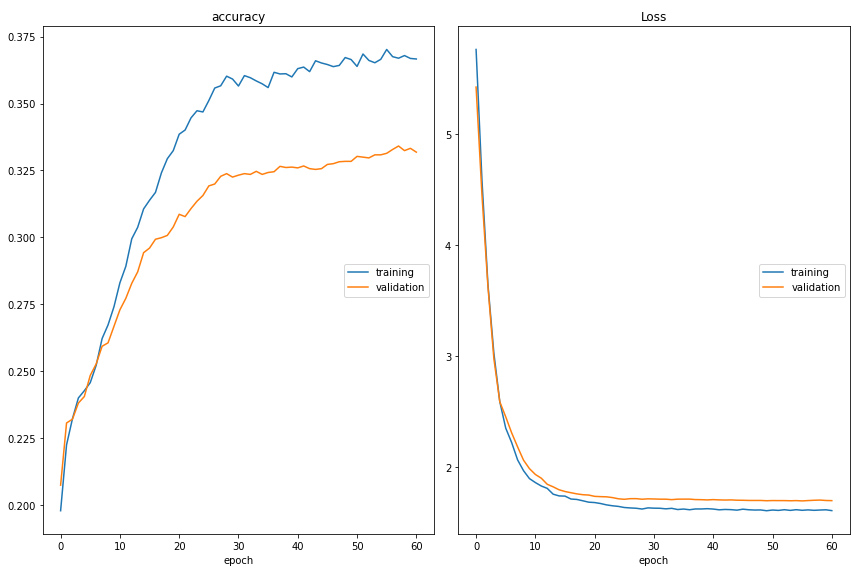
\includegraphics[width=0.6\textwidth]{figures/model/vgggraph.jpg}
    \caption{Training results of VGG-19 model}
    \label{fig:vgggraph}
\end{figure}
\noindent
We first stopped the training at 20 epochs, the plots didn't converge yet and it showed promise. We redid the training with 60 epochs and it appears that we assumed wrong. The loss is high at 1.6 and both training and validation accuracy are low at 36.6\% and 33.3\% and they stabilized in this range. This is another case of overfitting.
\subsection{Resnet-50}
\begin{figure}[H]
    \centering
    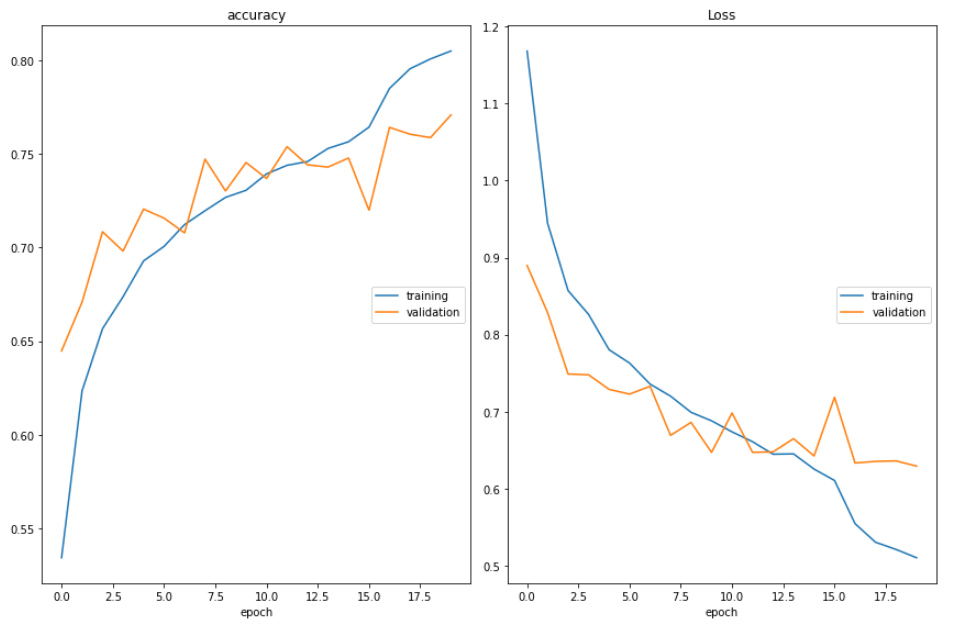
\includegraphics[width=0.6\textwidth]{figures/model/resnetgraph.jpg}
    \caption{Training results of Resnet-50 model}
    \label{fig:resnetgraph}
\end{figure}
\noindent
The training accuracy kept increasing and reached 81.1\% but the validation accuracy is fluctuating and don't follow the training curve. We remark a similar behaviour for the loss. While the validation accuracy is high around 75.6\%, we can safely assume that this model is overfitting and just does well on the test images.

\addtocontents{toc}{\protect\newpage}
\section{Results}
\subsection{Comparative Analysis}
\autoref{tab:models} puts the metrics of each model training against each other. Resnet-50 has the best metrics but it falls into overfitting. VGG-19 got the worse results. The coursera model is overall the best model to train our cleaned FER2013 dataset. We decided to use it but we need to optimize it and test it first.

\begin{table}[H]
\centering
\begin{tabular}{|c|c|c|c|c|}
\hline
\textbf{Model} & \textbf{Coursera} & \textbf{DeepFace} & \textbf{VGG-19} & \textbf{Resnet-50} \\
\hline
\textbf{Training accuracy} & 61.6\% & 59.9\% & 36.6\% & 81.1\% \\ 
\hline
\textbf{Validation accuracy} & 59.2\% & 54.2\% & 33.3\% & 75.6\%\\ 
\hline
\textbf{Training loss} & 1.02 & 1.07 & 1.6 & 0.51 \\ 
\hline
\textbf{Validation loss} & 1.05 & 1.2 & 1.69 & 0.63 \\
\hline
\textbf{Overfitting?} & \cellcolor{green!25}No & \cellcolor{red!25}Yes & \cellcolor{red!25}Yes & \cellcolor{red!25}Yes \\ 
\hline
\end{tabular}
\caption{Comparison of model training results}
\label{tab:models}
\end{table}

\subsection{Optimization and testing}
\subsubsection{Optimization}
We ran numerous trainings where we changed a single hyper-parameter each time to study its effect on the performance of the model, mainly batch size and learning rate.
We finally settled on a batch size of 16 and a learning rate of 0.00005. We  trained the model one final time for 250 epochs and \autoref{fig:finalgraph} shows the results.
\begin{figure}[H]
    \centering
    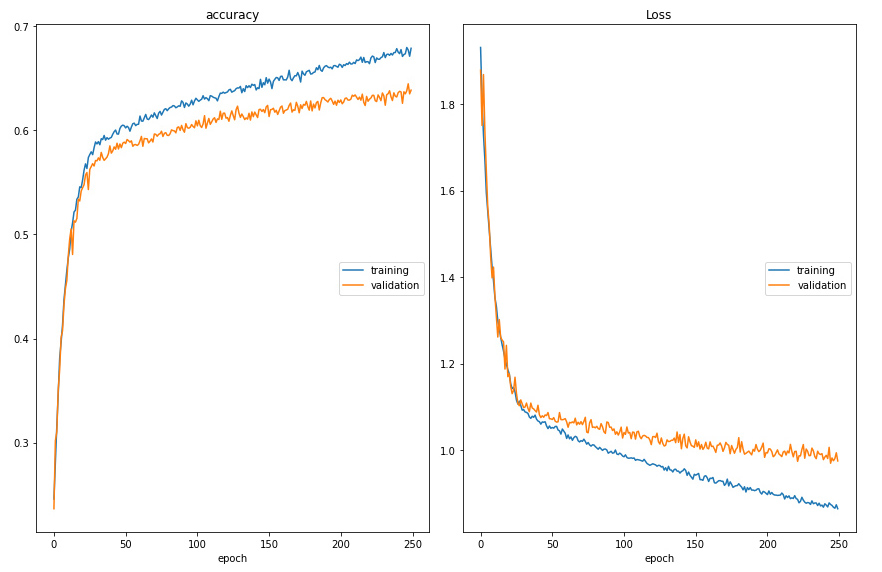
\includegraphics[width=0.55\textwidth]{figures/model/finalgraph.jpg}
    \caption{Final training results of Coursera model}
    \label{fig:finalgraph}
\end{figure}
\noindent
We obtained 67.89\% training accuracy and 63.87\% validation accuracy which is better than our first training with coursera model. We wanted to reach at least 70\% accuracy but this is an acceptable result.
\subsubsection{Testing}
To further understand our results, we generated a confusion matrix of the predictions on the test dataset. Confusion matrix is a useful visualization that confronts predicted labels against true labels and see how our model is really performing.
\begin{figure}[H]
    \centering
    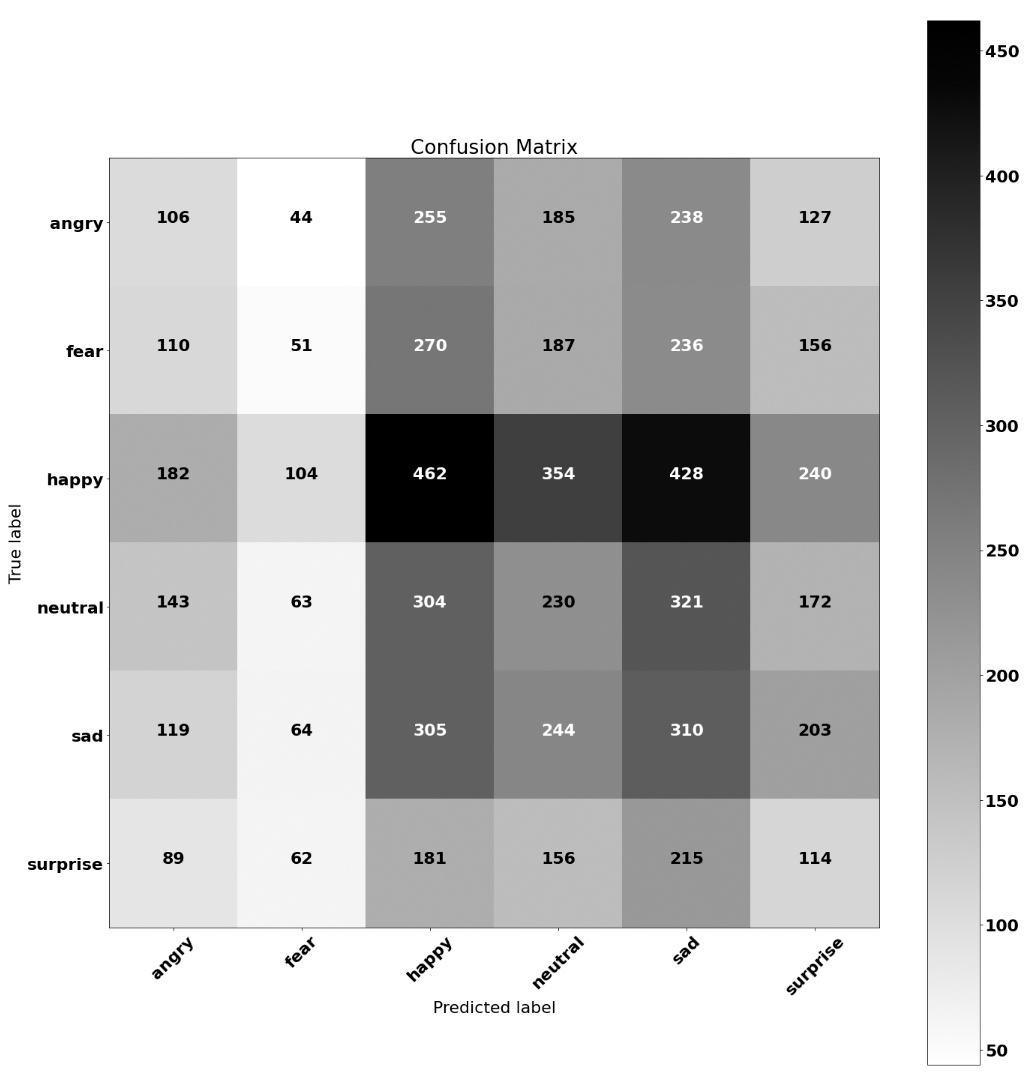
\includegraphics[width=0.6\textwidth]{figures/model/graph3.jpg}
    \caption{Confusion matrix}
    \label{fig:confusionmatrix}
\end{figure}
\noindent
Overall the expressions are correctly predicted. The happy expression is well detected but it also confuses it with the sad expression. This is because happy takes a big portion of the dataset. The fear expression is the least recognized expression because its features are less apparent than other expressions.
\\
We also used OpenCV and Flask to make a small testing application that outputs the predicted expression near a face captured by the laptop's webcam. \autoref{fig:opencvpics} shows the 6 expressions in action.
\begin{figure}[H]
    \centering
    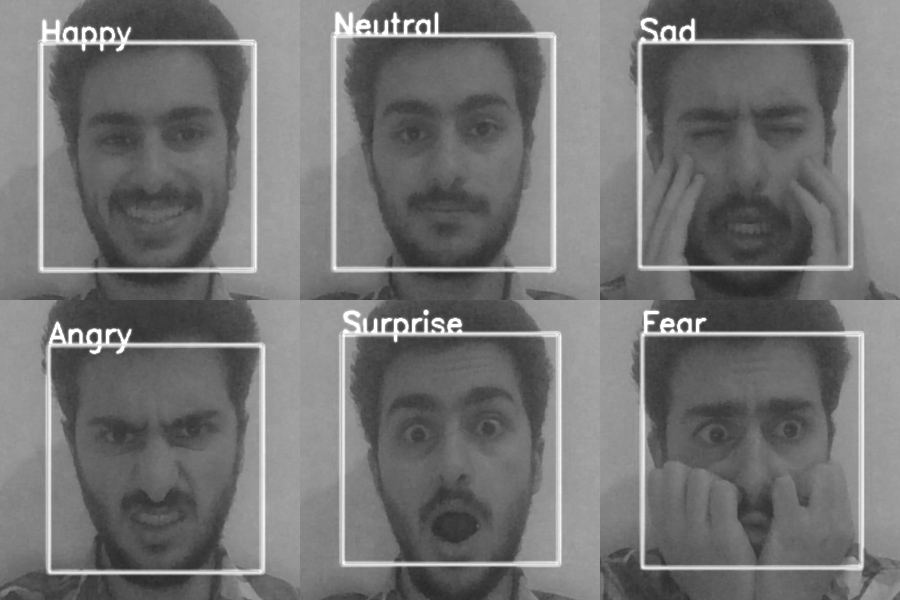
\includegraphics[width=0.6\textwidth]{figures/model/opencvpics.jpg}
    \caption{6 predicted expression with OpenCV}
    \label{fig:opencvpics}
\end{figure}

\section*{Conclusion}
In this chapter, we started dealing with the technical side of the project. We used Python and Keras to train the models in Google Colab. Then we chose the FER2013 dataset, cleaned it by removing wrong images and applied data augmentation on it. We trained 4 models and chose the Coursera model because it didn't overfit and we got 63.87\% validation accuracy after optimising it. We will present the browser extension where we used this model in the next chapter.

\chapter{Browser Extension Implementation}
\label{ch:4eme}
\minitoc
\newpage
\section*{Introduction}
After reaching a high accuracy model we now move on to the last step of our project which is the implementation of our pre-trained model into the browser. We have decided to implement the model via a Chrome extension that reads a video from the current web page, detects faces on that particular video and sends them to our pre-trained model to get the predictions. Finally, prediction results will be shown real time in the extension popup tab.

\section{Used Technologies}
In this section, we describe our development environment of choice and what technologies
we will be using in order to build the Chrome extension.
\subsection{Software environment}
We mainly used Visual Studio Code to implement the different components that our extension need. Visual Studio Code \cite{VisualStudioCode} is a lightweight but powerful source code editor which runs on your desktop and is available for Windows, Mac OS and Linux. It comes with built-in support for JavaScript, TypeScript and Node.js and has a rich ecosystem of extensions for other languages and runtimes.
\subsection{Used technologies}
We will present the main technologies we used to build the extension.
\begin{itemize}
\item NodeJS \cite{NodeJS}: NodeJS is a runtime environment for using server-side JavaScript. Thanks to its non-blocking operation, it allows the design of powerful networked applications, such as a web server, an API or a CRON job.
\item Tensorflow JS \cite{tfjs}:TensorFlow.js is an open-source hardware-accelerated JavaScript library for training and deploying machine learning models. It uses flexible and intuitive APIs to build models from scratch using the low-level JavaScript linear algebra library or the high-level layers API. It can execute native TensorFlow with the same TensorFlow.js API under the Node.js runtime. We can also use TensorFlow.js model converters to run pre-existing TensorFlow models right in the browser or even retrain pre-existing ML models using sensor data connected to the browser or other client-side data
\item Face-Api.js \cite{faceapi}: face-api is a JavaScript library created by Vincent Mühler., to detect faces via browser. It is built over tensorflow.js core API. It supports Face Detection, Face Recognition, Face Expression, Age, and Gender Detection
\end{itemize}
\section{Realisation}
\subsection{Chrome extension}
There are 3 major components to build a Chrome extension:
\begin{itemize}
\item The manifest file : 
This is the ledger of a chrome extension. It's a JSON file that describes the behavior of a Chrome extension. You list things like your extensions name, a description, which files or libraries you're including, and the permissions your extension needs.
\begin{figure}[H]
    \centering
    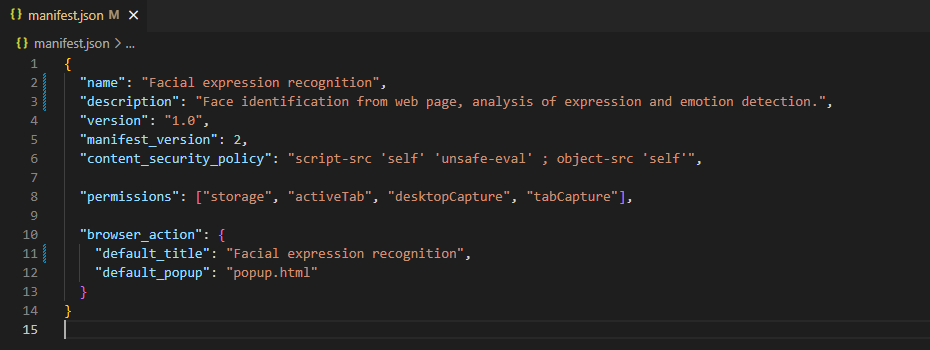
\includegraphics[width=0.7\textwidth]{figures/manifest.png}
    \caption{Manifest.json file}
    \label{fig:manifestfile}
\end{figure}
\item Background.js : 
We can think of it as the backend of our project. It is a JavaScript script that runs once our extension either gets installed or the user refreshes the extension manually and contains all the logic. 
\item Popup.html : 
This is a HTML page that users see when they click on the extension icon in the menu bar.
This is one of the ways users can interact with our extension like a front-end.
\end{itemize}

\subsection{Implementation Steps}
After building the manifest and popup files we focus on the logic of the project. Here are the different steps we implemented to get our model working in a chrome extension : 
\begin{itemize}
\item Convert our FER model into a web friendly format using tf js-converter. This conversion produces 2 files. A JSON file which contains the dataflow graph and a weight manifest file and a group1-shard of files which are a collection of binary weight files.
\item We load our converted model.json from a distant server using Tensorflow JS's loadLayersModel API. This asynchronous function also automatically detects the binary weight files from the same directory of the model. The return value of tf.loadLayersModel is tf.Model.
\begin{figure}[H]
    \centering
    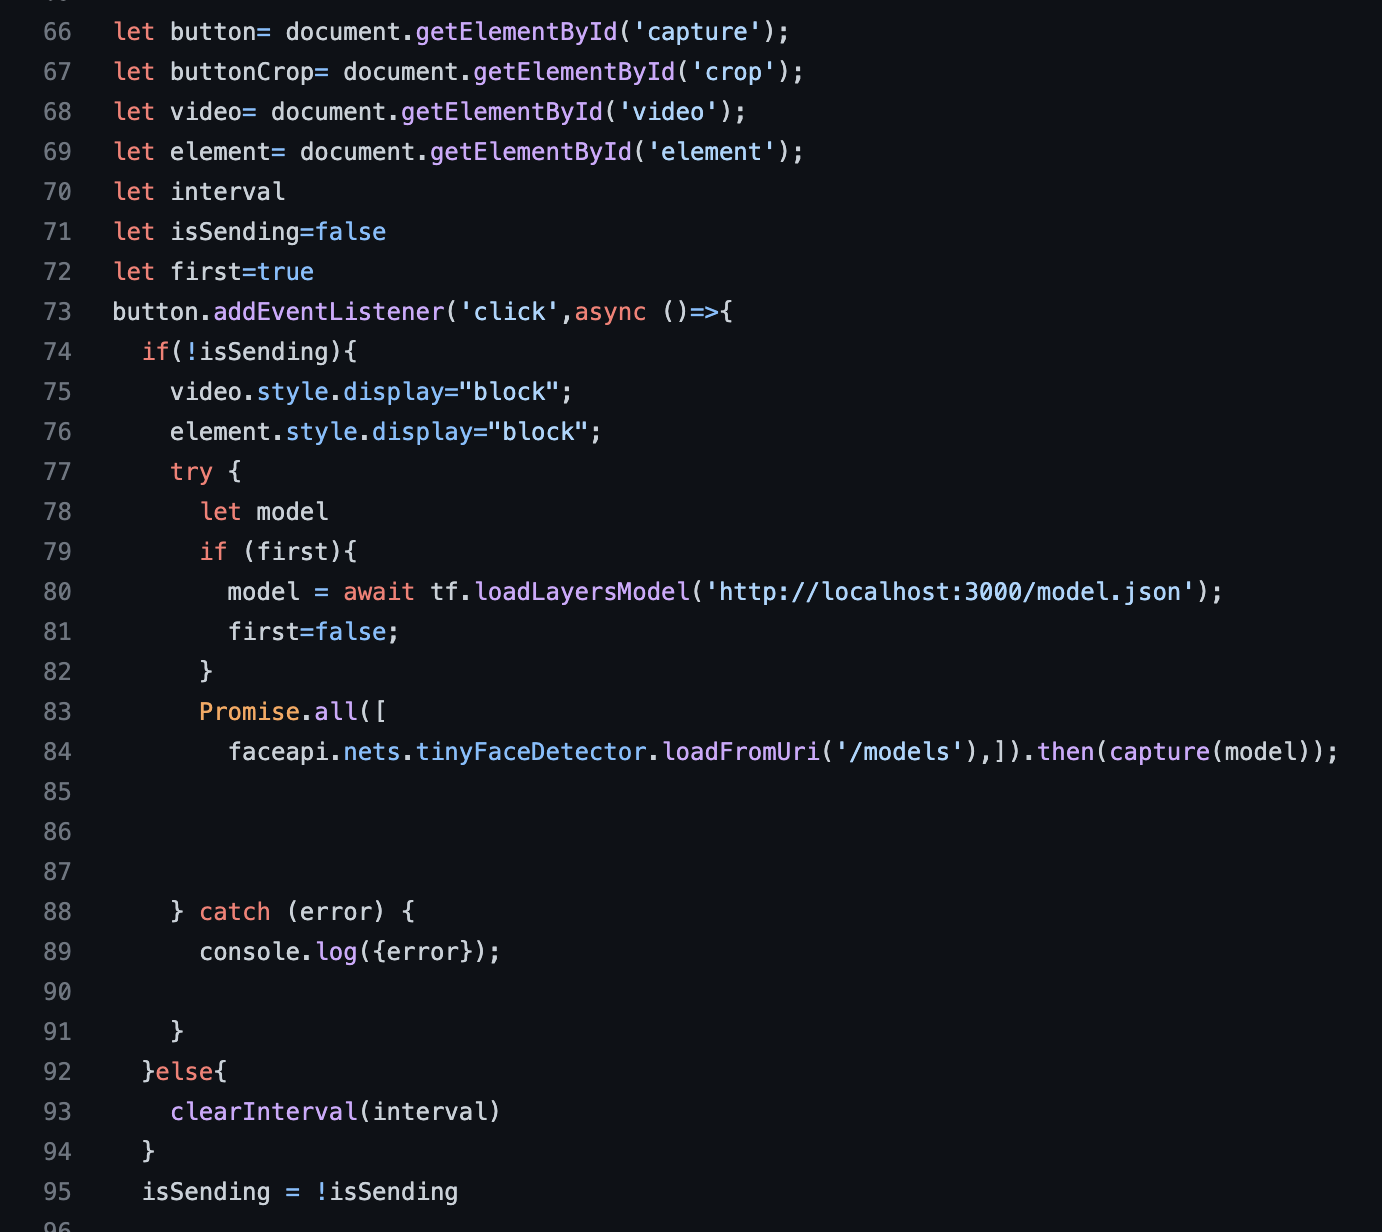
\includegraphics[width=0.7\textwidth]{figures/LoadingModels.png}
    \caption{Loading Models}
    \label{fig:loadingmodels}
\end{figure}
\item We used a chrome extension tool “chrome.tabCapture()“ to capture the video from web page and display it into the extension.
\item We proceed to detect the faces from the captured video using face-api.js. This returns image frames of all faces if they exist in the video.
\begin{figure}[H]
    \centering
    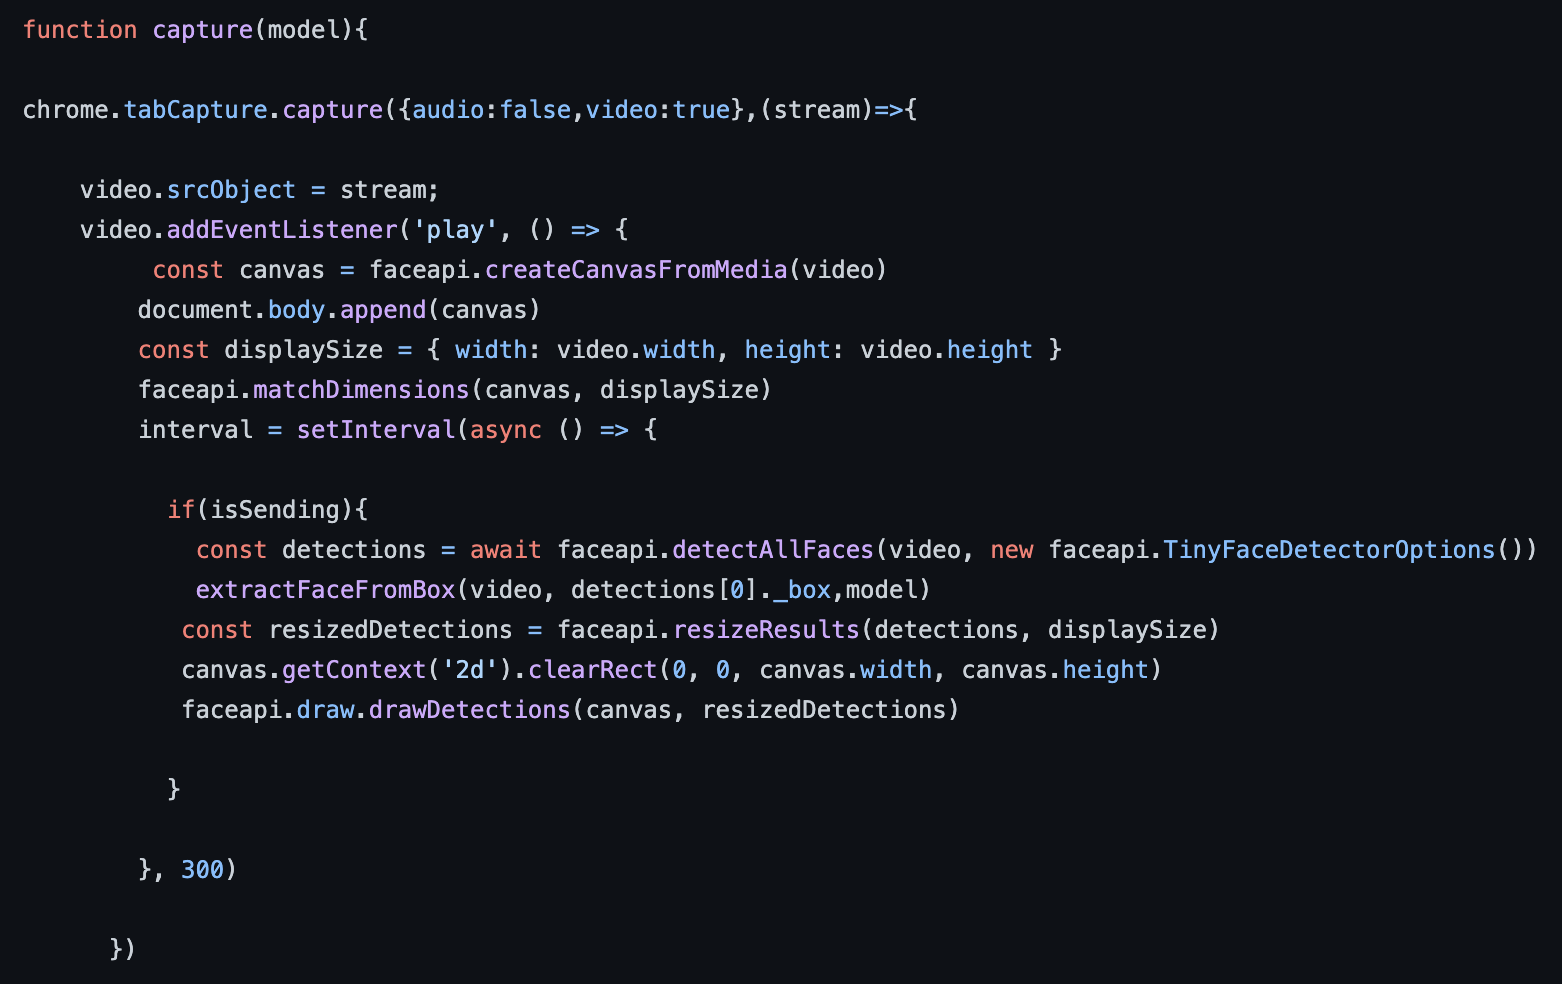
\includegraphics[width=0.7\textwidth]{figures/CapturingVideo.png}
    \caption{Detecting Faces from Video}
    \label{fig:facedetection}
\end{figure}
\item We now proceed to match the image frames with the model input by grayscaling and resizing them into 48x48 pixel images.
\item We send to the loaded model the resized images as a canvas using the predict() function from Tensorflow JS which will produce the output estimates for the given input instances.
\begin{figure}[H]
    \centering
    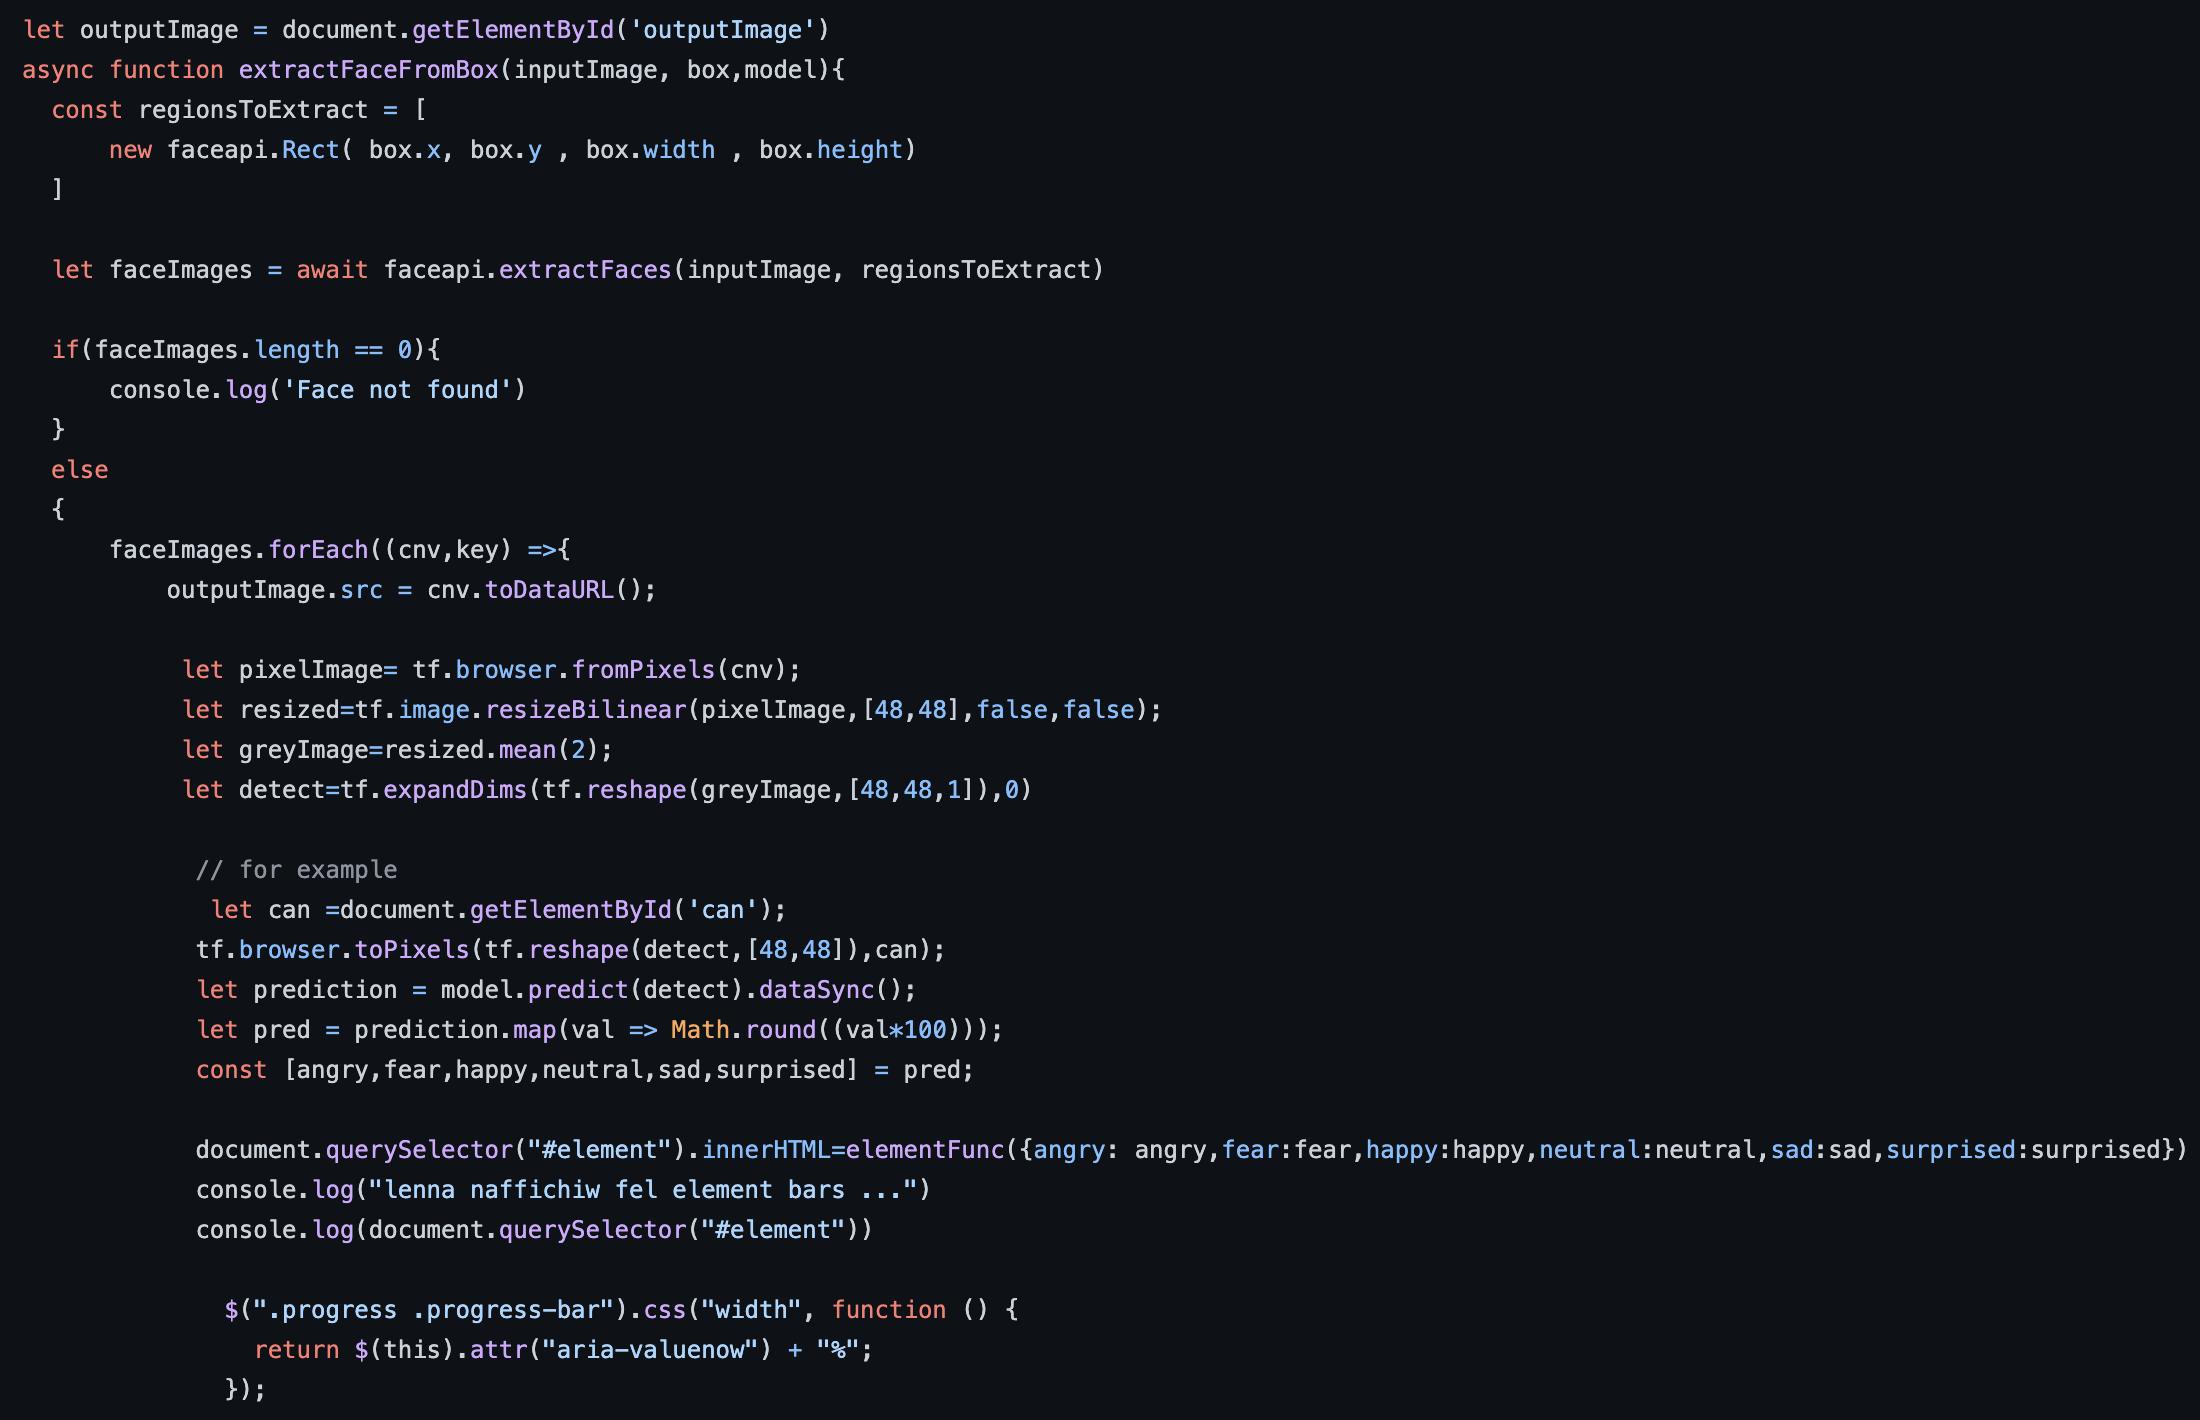
\includegraphics[width=0.7\textwidth]{figures/Resize&predict.png}
    \caption{Manipulating Image and Predicting}
    \label{fig:resizingandpredicting}
\end{figure}
\item Finally, we utilize the output and display it to the user on the popup page of the extension.
\end{itemize}
\begin{figure}[H]
    \centering
    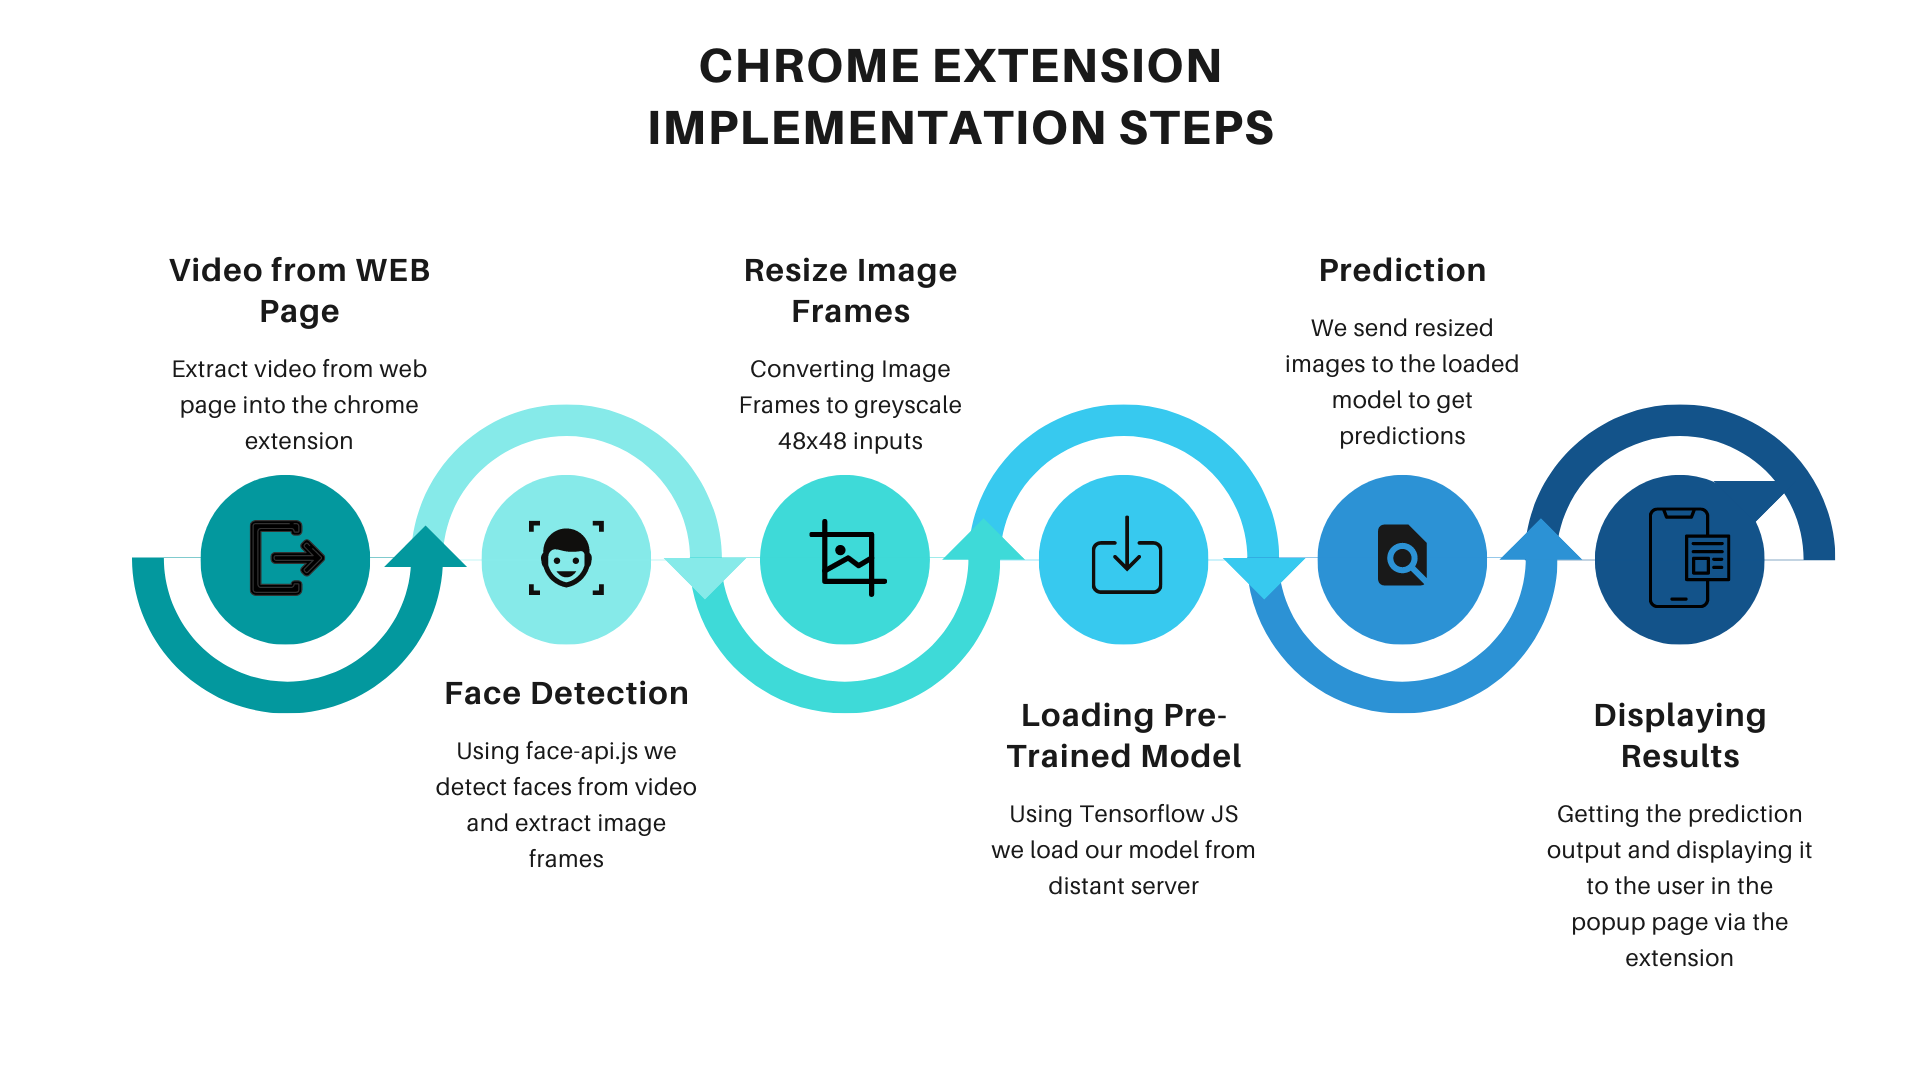
\includegraphics[width=0.7\textwidth]{figures/steps.png}
    \caption{Implementation Steps}
    \label{fig:implementationsteps}
\end{figure}
\subsection{Interface}
The extension interface is depicted in \autoref{fig:browserinterface} below. To use it, the user needs to install it in his Google Chrome browser then when he wants to apply it on a video he is watching or in a video-call, he can activate the extension and click on the "Start" button.
The popup will start detecting the face live and predict the emotions on the side. The dominant expression is shown with the percentages of each emotion below it in progress bars. The predictions are done real-time so progress bar can increase and decrease accordingly. The user can pause the process on a given frame by clicking on the "Pause" button.

\begin{figure}[H]
\begin{center}
\subfloat[]{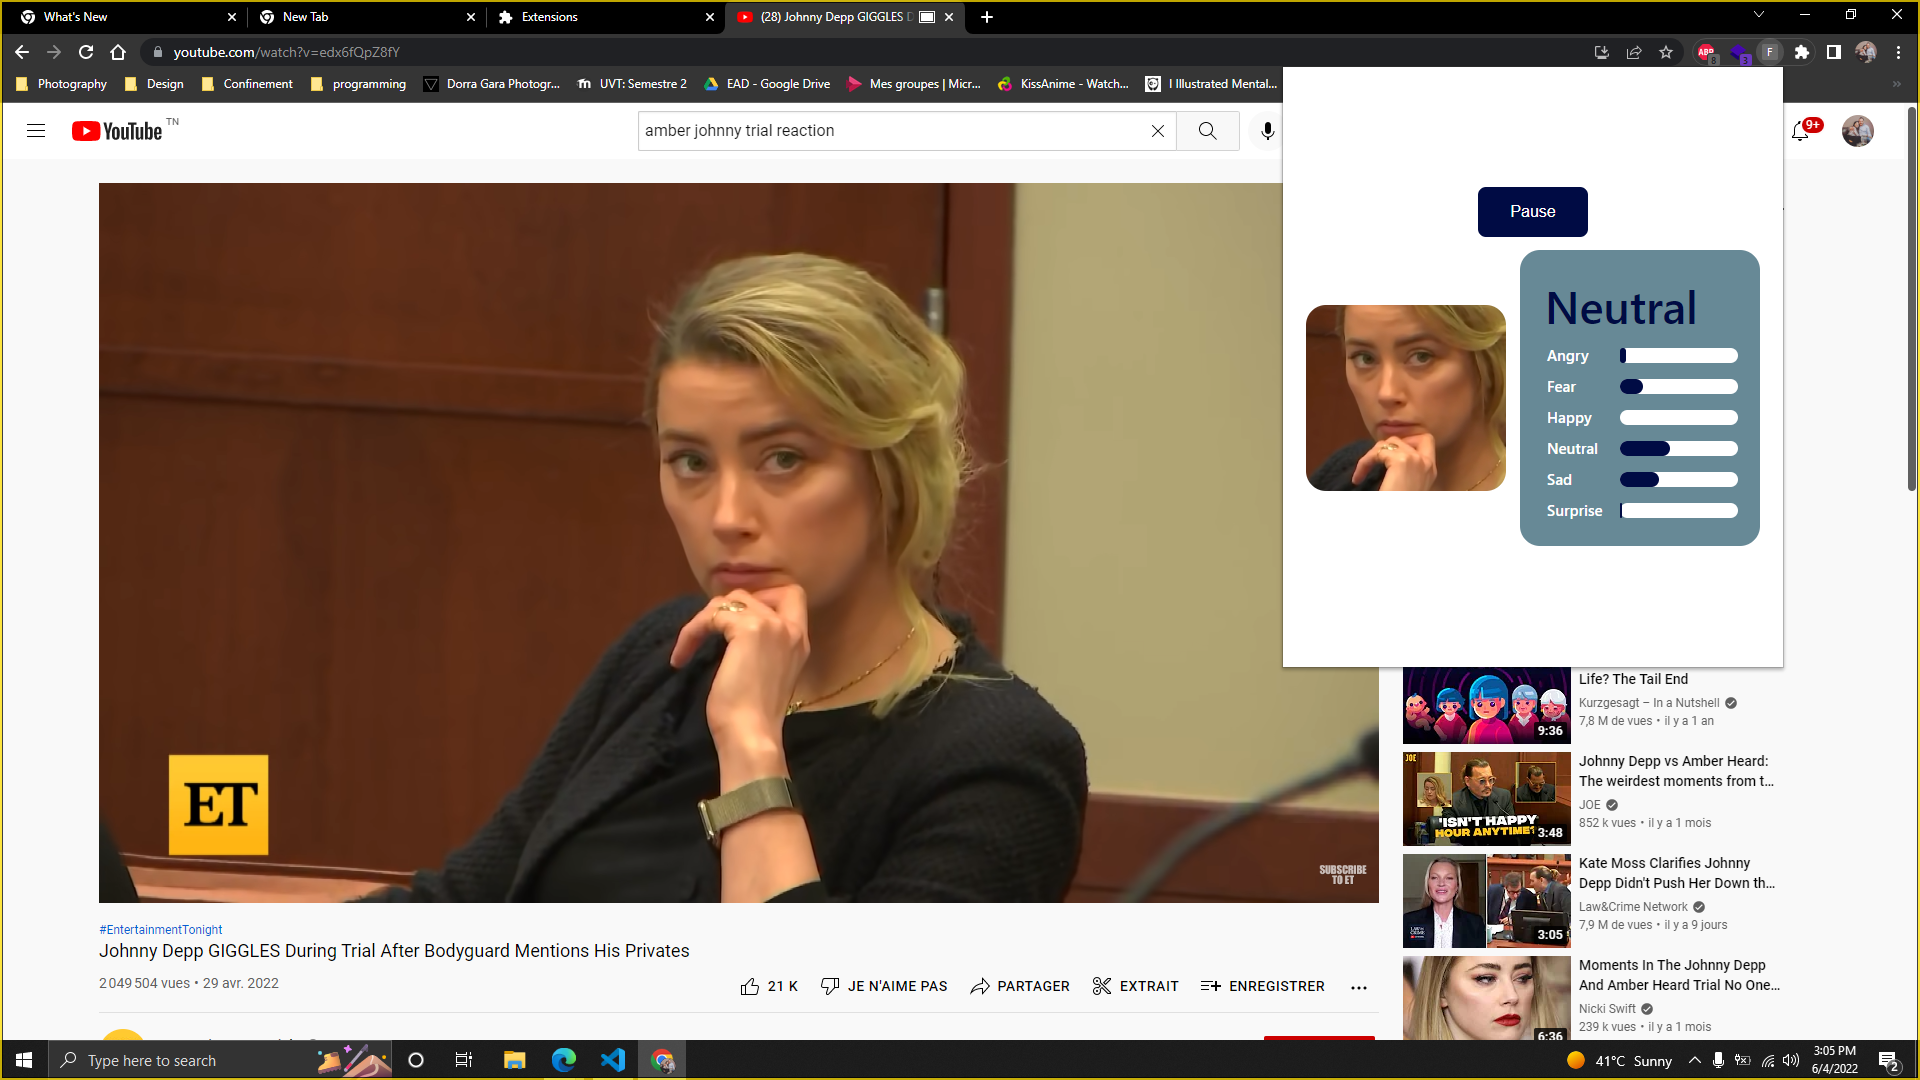
\includegraphics[width=0.4\textwidth]{figures/model/interface2.png}} 
\subfloat[]{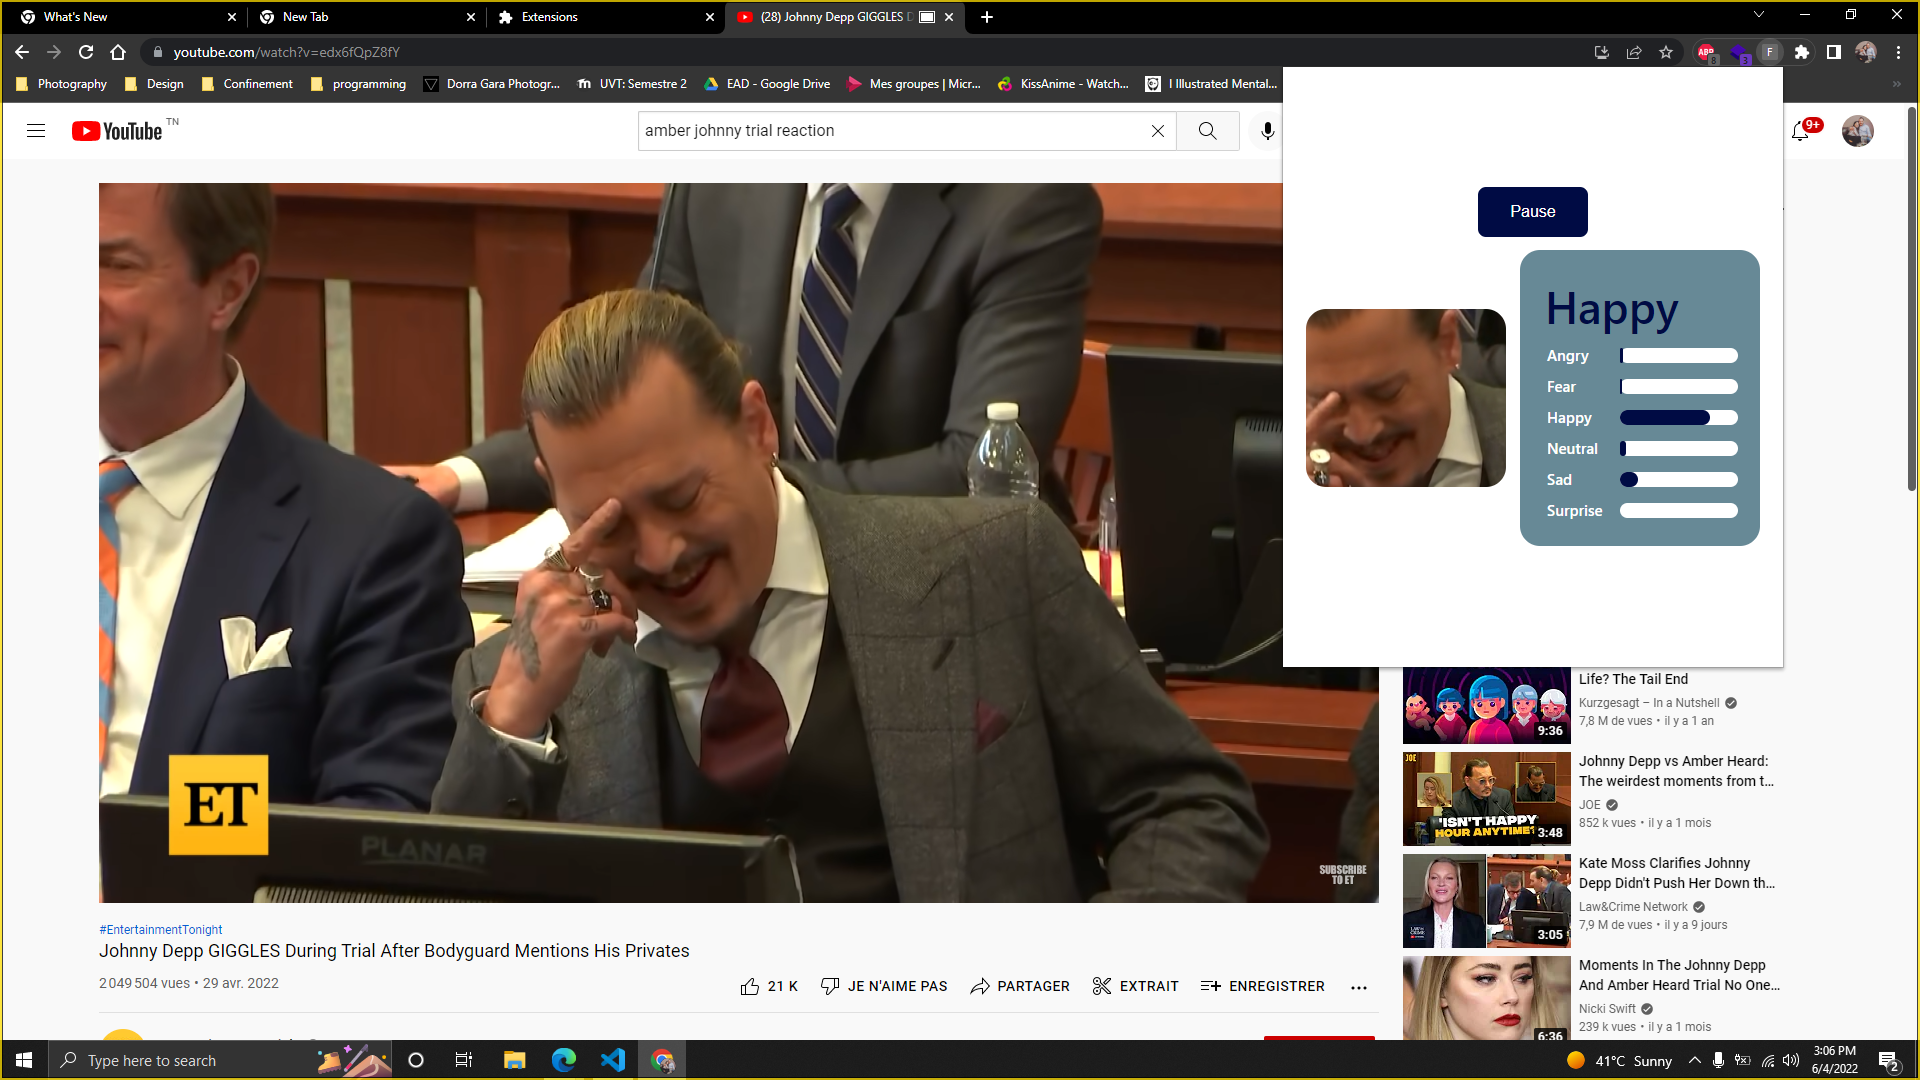
\includegraphics[width=0.4\textwidth]{figures/model/interface4.png}}\quad
\subfloat[]{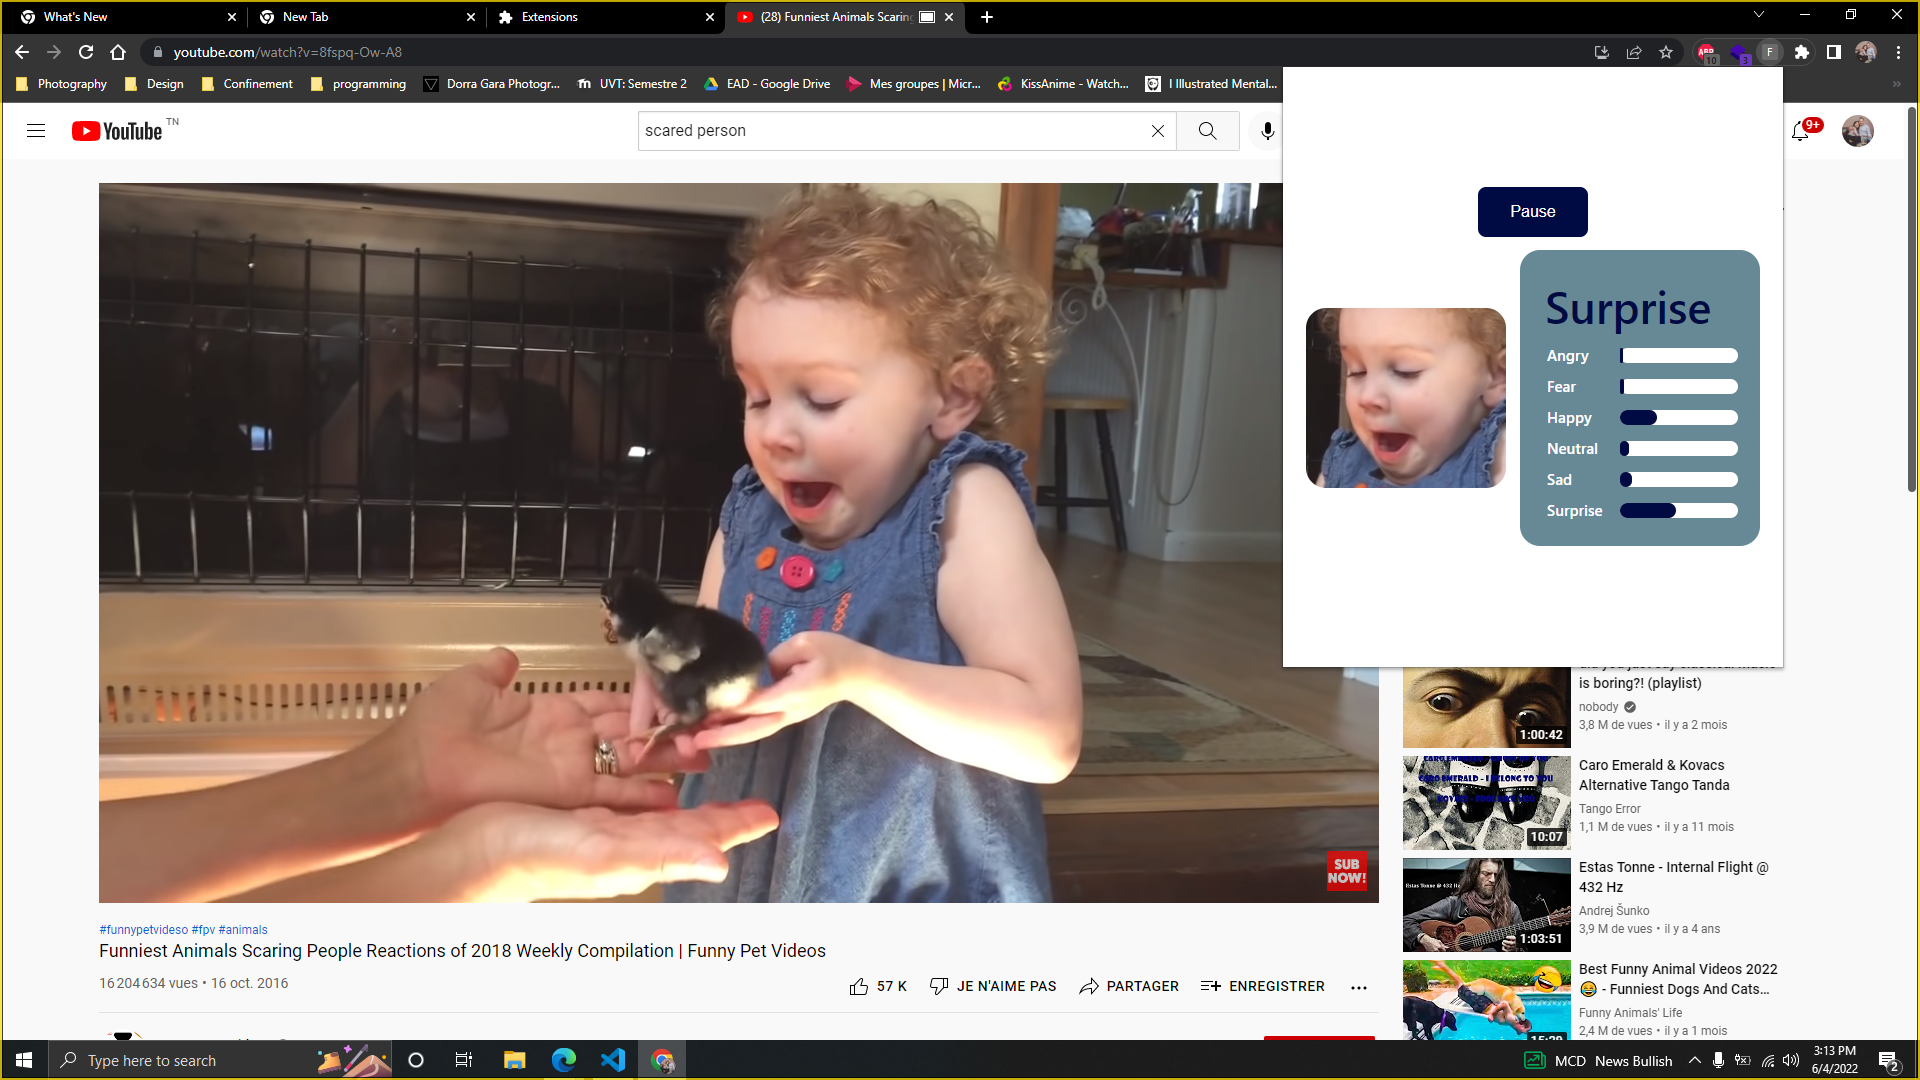
\includegraphics[width=0.4\textwidth]{figures/model/interface3.png}}
\subfloat[]{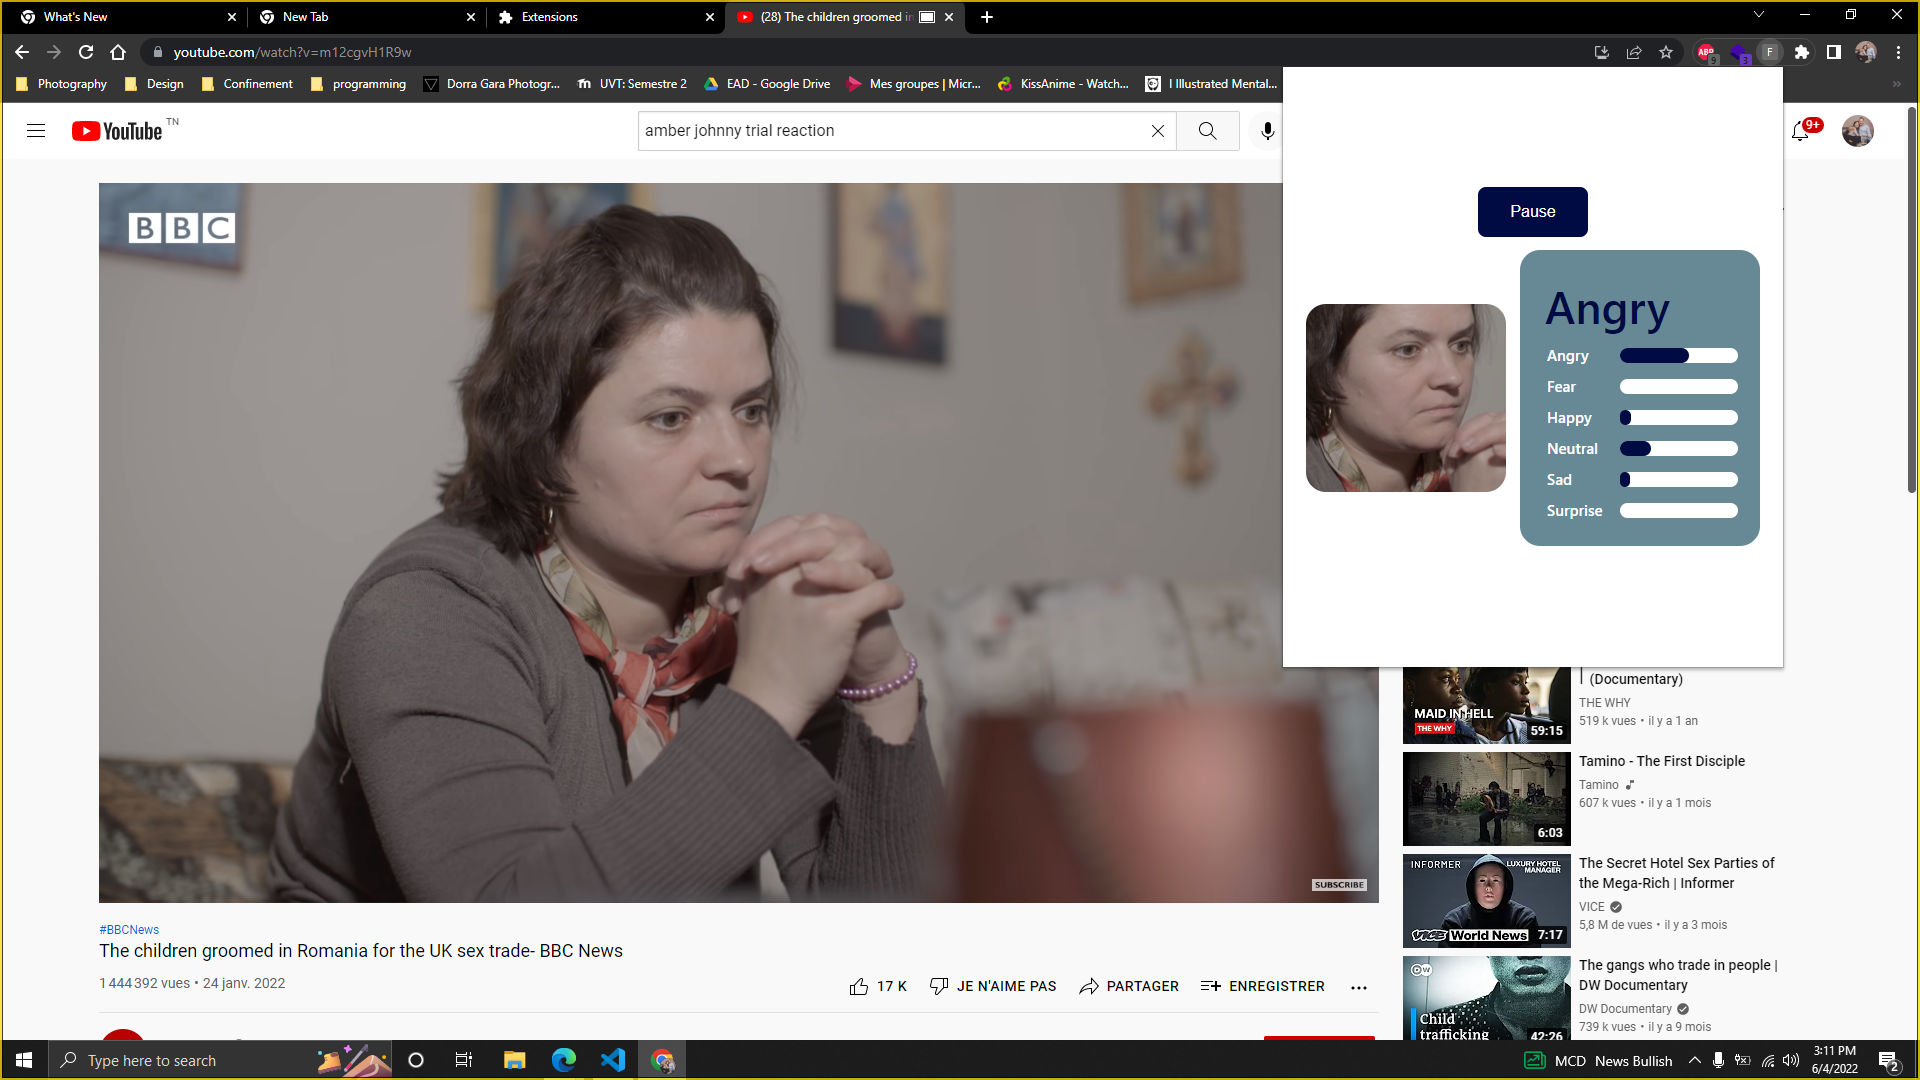
\includegraphics[width=0.4\textwidth]{figures/model/interface1.png}}
\caption{Interface of our Chrome extension}
\label{fig:browserinterface}
\end{center}
\end{figure}


\section*{Conclusion}
This chapter gave us an insight on how to build a chrome extension from scratch and especially on how to implement a machine learning Pre-trained model on the browser using the Tensorflow JS library. We also presented the interface and how it works to detect the emotions.

\chapter*{\textbf{Conclusion and perspectives}}
\addcontentsline{toc}{chapter}{Conclusion and perspectives}
\markboth{Conclusion and perspectives}{}
\lettrine[findent=2pt]{\textbf{E}}{ }xpressions reveal what takes place within the human mind at a time. They are the key to understand the feelings of an interlocutor thus improving the communication.
Nowadays, computer vision and deep learning are enabling us to derive meaningful information from digital images, automating the process of recognition and answering to complex challenges.\\ \\
\indent It is within this framework, our end of year project revolved around using these technologies for facial expression recognition. As a first step, we started by studying the concept behind Convolution Neural Networks and the layers that composes it. We also found and compared 4 possible datasets for training our model. \\
\indent As a second step, we searched and stated the existing models and implementations. We found 4 models, 2 with CNN and 2 with transfer learning, that were used in FER. We also found 4 solutions that delivers different use cases of FER in different platforms (browser extension, surveillance system, mobile application, video editor). This made our goals clear to train a model and implement it in a browser extension.\\
\indent As a third step, we studied the datasets and we chose the FER2013 because it is accessible and has a high number of images. We then cleaned it and augmented it. We trained 4 models on it and the Coursera model got the best performances without overfitting. We optimized it and reached 63.87\% accuracy.\\
\indent As a final step, we wanted to offer the possibility for every user to analyze the emotions of an interlocutor so we implemented our model into a Chrome extension so that users can either detect the expressions of a speaker from a youtube video or a video call.
\newpage
\indent In terms of perspective, we propose adding another Deep Learning model that integrates voice emotion recognition to evolve our emotional analysis. This can be accomplished by detecting voice from audio, predicting its emotion and pairing it with our FER prediction for pertinence. With more time we are able to improve our model's accuracy and the extension general performance. We can even further develop our browser extension to hold more features based on these analysis, like profiling and even lie detection.

\spacing{1.1}
\begin{flushleft}
    \bibliographystyle{unsrt}
    \bibliography{references}
\end{flushleft}

\end{document}